% ------------------------------------------------------------
% This is a template for technical reports
% The Main_thesis.txt is the master control file. It is like the
% main function in a C code. Here we use it to load individual chapters.

% Author: Pham Hung Thinh, NTU, Singapore
% Date: 12, 2012
% Template from: Xiao Xiong, NTU, Singapore
% ------------------------------------------------------------


%----------------------------------------------------------------------------
% File          PpHd.tex
% Author        Ong Kok Leong
% Description   preamble: the global settings
%-----------------------------------------------------------------------------

% 1. Define your report format here
\documentclass[12pt,a4paper,twoside]{report}

% 2. Specify the packages to be included
\usepackage{graphicx}
\usepackage{subfigure,amssymb,amsmath,epsfig,fancyheadings,citesort}
\usepackage{times,eqnarray,amsmath,epsfig}
\usepackage{pgfplots}
\pgfplotsset{compat=1.5}
\usepackage{todonotes}
\usepackage{booktabs}

\usepackage{tikz}
\usepackage{xcolor}	
\usepackage{makecell}
\usepackage{slashbox}
\usetikzlibrary{arrows, positioning, calc}

\oddsidemargin  +0.10in %
\evensidemargin +0.00in %
\topmargin      +0.15in %
\textheight     +8.50in %
\textwidth      +6.25in %

\pagestyle{plain}

\font\Bold=cmbx10 scaled \magstep3
\def\EndOfProof{\nolinebreak\ \hfill\rule{1.5mm}{2.7mm}}
\def\endOfProof{\ \hfill\rule{1.5mm}{2.7mm}}

\def\proof{\noindent \textbf{Proof:}\quad}

%\renewcommand{\theequation}{\mbox{\rm Eq.\ \thechapter.\arabic{equation}}}

\newcounter{theorem}
\newtheorem{theorem}{Theorem}
\renewcommand{\thetheorem}{\thechapter.\arabic{theorem}}

\newcounter{lemma}
\newtheorem{lemma}{Lemma}
\renewcommand{\thelemma}{\thechapter.\arabic{lemma}}

\newcounter{corollary}
\newtheorem{corollary}{Corollary}
\renewcommand{\thecorollary}{\thechapter.\arabic{corollary}}

\newcounter{definition}
\newtheorem{definition}{Definition}
\renewcommand{\thedefinition}{\thechapter.\arabic{definition}}

\newcounter{algo}
\newtheorem{algo}{Algorithm}
\renewcommand{\thealgo}{\thechapter.\arabic{algo}}

\renewcommand{\thefigure}{\thechapter.\arabic{figure}}
\renewcommand{\thesubfigure}{\thefigure.\alph{subfigure}}
\makeatletter
\renewcommand{\@thesubfigure}{\thesubfigure:\space}
\renewcommand{\p@subfigure}{}

\def\LEQ.#1.#2.#3{#1\!\leqslant\!#2\!\leqslant\!#3}
\def\GEQ.#1.#2.#3{#1\!\geqslant\!#2\!\geqslant\!#3}
\def\emptyset{\varnothing}
\renewcommand{\theenumi}{\rm \roman{enumi}}
\renewcommand{\labelenumi}{\rm (\theenumi)}
\renewcommand{\theenumii}{\rm \alph{enumii}}
\renewcommand{\labelenumii}{\rm (\theenumii)}

\renewcommand{\topfraction}{0.75}
\renewcommand{\bottomfraction}{0.75}
\renewcommand{\textfraction}{0.10}

%
% Report specific definitions
%

%
% Definition in the context of this report.
%
\def\reporttitle    {An Algorithmic Framework for Web Data Mining}
\def\supp           {\varphi}
\def\psupp          {\varphi^{\mathcal{P}}}
\def\conf           {\delta}
\def\pconf          {\delta^{\mathcal{P}}}
\def\tab            {\hspace{0.8cm}}

%
% Define the set of symbols for the constraint set.
%
\def\map            {\Pi}
\def\gen            {\Upsilon}
\def\prune          {\Phi}
\def\selcand        {\Psi}
\def\compute        {\Theta}
\def\check          {\Omega}

%
% The set of operators
%
\def\select         {\sigma}
\def\proj           {\pi}
\def\join           {\bowtie}
\def\apply          {\mu}
\def\undo           {\eta}
\def\rename         {\leftarrow}

\def\linespaceNormal        {\baselineskip=24pt}
\def\linespaceTight         {\baselineskip=21pt}
\def\linespaceVeryTight     {\baselineskip=19pt}

\renewcommand{\bibname}{References}

% Define some new macros
%\def\addnotation #1: #2#3{$#1$\indent \parbox{5in}{#2 \dotfill  \pageref{#3}}}
\def\addnotation #1: #2#3{$#1$ & #2 & \pageref{#3}}
\def\newnot#1{\label{#1}}
     % Input Global settings




\begin{document}    % Start of the text



% -------------------------------------------------------------------------------- %
% --------------------------- Part I. Front Matters ------------------------------ %
% -------------------------------------------------------------------------------- %

\title{\sc
\resizebox*{0.5\textwidth}{!}{
\includegraphics{NTU_new_logo.eps}}\\[3em]
\vspace{-0.5in}Power Optimisation for Adaptive Embedded Wideband Radios  \\
\vspace*{0.3in} \centering
}

\author{
A Thesis submitted to\\
the School of Computer Engineering\\
of Nanyang Technological University\\[1em]
by\\[1em]
{\rm\bf Pham Hung Thinh}\\[1.5em]
in fulfillment of the requirement for \\
the Degree of Doctor of Philosophy of\\
for Computer Engineering\\[1.5em]
}

\date{\today}
\maketitle
\thispagestyle{empty}        % no page number on this front cover page
       % Input the Cover page

\setlength{\baselineskip}{20pt plus 1pt minus 1pt} % Use 1-1/2 spacing for whole document
\pagenumbering{roman}   % Use small roman digits for the page number of front matters

%\chapter* {Abstract}
\addcontentsline{toc}{section}{\numberline{}\hspace{-0.35in}{\bf
Abstract}}  % Add the Abstract to the table of contents using the specified format

The thesis explores techniques for enabling cognitive radio design on field programmable gate arrays (FPGAs). We demonstrate the strengths of FPGAs in offering a high throughput, low-power baseband platform, and develop a flexible Orthogonal Frequency Division Multiplexing (OFDM) baseband chain with high-level control and support for multiple standards. We present contributions in OFDM synchronisation to enable more robust radios in harsher channels, and tolerating less precise RF components. We also present a novel technique for managing out of band leakage to enable more efficient spectral use in a dynamic spectrum allocation setting. For each of these approaches, we design, optimise, and characterise working hardware implementations of the required modules, with a focus on flexibility and low power. Finally, we present an approach for applying FPGA partial reconfiguration to minimise reconfiguration time when a radio switches modes, allowing intermediate data to be buffered and processed after reconfiguration is complete. These contributions form an important foundation in building a fully functional prototyping platform for cognitive radio systems.    % Input the abstract and acknowledgement
%\chapter* {Acknowledgments}
\addcontentsline{toc}{section}{\numberline{}\hspace{-.35in}{\bf Acknowledgments}}

It is great pleasure to me in expressing my gratitude to all those people who have continuously
supported me and had their contributions in making this thesis possible.

I would like to express my sincere thanks and appreciation to my supervisors, Prof. Suhaib Fahmy, and Prof. Ian McLoughlin for giving me constant trust during the entire research of my Ph.D. studies, for their helpful suggestions and advices, for their continuous support and their teachings essential to achieve this objective.

I express my sincere gratitude towards Prof. Samarjit Chakraborty at Institute for Real-Time Computer Systems, TU Munich for providing me an internship opportunity in the final stage of my PhD.

I also wish to thank all colleagues and technical staffs in CHiPES for their prompt support and helpful in providing all the facilities required for my research work.


Last but not least, I would like to acknowledge my family in Viet Nam, for their constant love and encouragement.
	

\newpage
\setcounter{secnumdepth}{3} % section numbering depth
\setcounter{tocdepth}{2}    % count to the depth of sections
\tableofcontents            % table of contents appears here

\newpage
\addcontentsline{toc}{section}{\numberline{}\hspace{-.35in}{\bf List of Figures}}
\listoffigures              % list of figures appears here

\newpage
\addcontentsline{toc}{section}{\numberline{}\hspace{-.35in}{\bf List of Tables}}
\listoftables              % list of tables appears here

%%\chapter* {List of Abbreviations}
%\addcontentsline{toc}{section}{\numberline{}\hspace{-.35in}{\bf List of Abbreviations}}
%\begin{tabular}{p{100pt}l}
\listofsymbols{ll}{
  % after \\: \hline or \cline{col1-col2} \cline{col3-col4} ...
ADC & Analogue to Digital Converter   \\
ASICs & Application Specific Integrated Circuits   \\
AWGN & Additive White Gaussian Noise   \\
AXI  & Advanced eXtensible Interface \\
BCU & Basic Channel Unit   \\
BER & Bit Error Rate   \\
BPSK & Binary Phase Shift Keying   \\
CFO & Carrier Frequency Offset   \\
CIR & Channel Impulse Response   \\
COTS & Commercial Off-The-Shelf   \\
CP & Cyclic Prefix   \\
CPE & Common Phase Error   \\
CR & Cognitive Radio   \\
DAC & Digital to Analogue Converter   \\
DFT & Discrete Fourier Transform   \\
DMT & Discrete Multi Tone   \\
DSA & Dynamic Spectrum Access   \\
DSP & Digital Signal Processing   \\
DSRC & Dedicated Short-Range Communications   \\
FBMC & Filter Bank Multi-Carrier   \\
FDM & Frequency Division Multiplexing   \\
FFO & Fractional Frequency Offset   \\
FFT & Fast Fourier Transform   \\
FPGA & Field Programmable Gate Array   \\
ICAP & Internal Configuration Access Port \\
ICI & Inter Carrier Interference   \\
IDFT & Inverse Discrete Fourier Transform   \\
IFFT & Inverse Fast Fourier Transform   \\
IFO& Integer Frequency Offset   \\
IQ & In-phase - Quadrature   \\
ISI & Inter Symbol Interference   \\
IUs & Incumbent Users   \\
LNA & Low Noise Amplifier   \\
%\end{tabular}
%\newpage %IVM added - this runs on below the end of the A4 page
%\begin{tabular}{p{100pt}l}
MAN & Metropolitan Area Networks   \\
MCM & Multi-Carrier Modulation   \\
MIMO & Multi-Input Multi-Output   \\
ML & Maximum Likelihood   \\
MPoC & Multiple Processors on Chip   \\
MSB& Most Significant Bit   \\
MSCRs & Multiple Standard Cognitive Radios   \\
MSE & Mean Squared Error   \\
NC-OFDM & Non-Contiguous Orthogonal Frequency Division Multiplexing   \\
OFDM & Orthogonal Frequency Division Multiplexing   \\
PAPR & Peak-to-Average Power Ratio   \\
PAR & Place And Route   \\
PDF & Probability Density Function   \\
PLL & Phase-Locked Loop   \\
PR & Partial Reconfiguration   \\
PUs & Primary Users   \\
QAM & Quadrature Amplitude Modulation   \\
QPSK & Quadrature Phase Shift Keying   \\
RF & Radio Frequency   \\
RTL & Register Transfer Level   \\
RTO & Residual Timing Offset   \\
RTV & Road to Vehicle   \\
SEM & Spectrum Emission Mask   \\
SER & Symbol Error Rate   \\
SNR & Signal to Noise Ratio   \\
STO & Symbol Timing Offset   \\
SUI & Stanford University Interim   \\
SUs & Secondary Users   \\
TVBD & TV Band Devices   \\
TVWS & Television White Spaces   \\
V2V & Vehicle-to-Vehicle   \\
WLAN & Wireless Local Area Networks   \\
XPA & Xilinx Power Analyzer   \\
XPE & Xilinx Power Estimator   \\
}
%\end{tabular}
      % Input the list of abbreviations and notations
%\chapter* {List of Notation}
\addcontentsline{toc}{section}{\numberline{}\hspace{-.35in}{\bf List of Notation}}

\begin{tabular}{p{70pt}p{330pt}}
    $\ast$ & Convolution\\
    $(\cdot)^T$ & Matrix or vector transpose \\
    $i$ 	& imaginary unit \\
   $|a|$ & absolute value of the number a \\
   $\angle{a}$ & argument of a complex number in $[0, 2 \pi]$ \\
   $\hat{a}$ 	& compensated for the parameter a \\
   $x(t)$ & time continuous signal \\
   $x[d]$ & time discrete signal; $d$ is time index \\
   $x[d]'$ &  offseted discrete signal \\
   $\widehat{x[d]}$ & compensated discreate signal \\
   $\Delta f_{C}$ & carrier frequency offset normalized to the intercarrier spacing \\
   $sinc(t)$ & $\triangleq \frac{sin(\pi t)}{(\pi t)}$ \\
   $(f * g)(m) $ &  $\triangleq \sum_{n} f(n)g(m - n)$ convolution product \\
\end{tabular}

%\addnotation \ast: {Convolution}{ast}\\
%\addnotation \otimes: {Kronecker product}{otimes}\\
%\addnotation (\cdot)^T: {Matrix or vector transpose}{transpose}\\
%\addnotation \bullet: {Elementary multiplication}{bullet}\\
%\addnotation \textrm{diag}(\textbf{x}): {Make a diagonal matrix whose diagonal elements are the elements of vector \textbf{x}}{diag}\\
%\addnotation ||\textbf{x}-\textbf{y}||^2: {Euclidian distance between \textbf{x} and \textbf{y}}{Euclidian}\\
%\addnotation |X|: {Determinant of matrix $X$}{determinant}\\
%\addnotation \textbf{x}\bullet\textbf{y}: {Element-wise multiplication of \textbf{x} and \textbf{y}}{element_multi}\\
%\addnotation \textbf{x}\bullet/\textbf{y}: {Element-wise division of \textbf{x} by \textbf{y}}{element_divide





% -------------------------------------------------------------------------------- %
% --------------------------- Part II.  The Body ---- ---------------------------- %
% -------------------------------------------------------------------------------- %
\addtolength{\headheight}{3pt} \pagestyle{fancy}
\setlength{\headrulewidth}{0.1pt}
\renewcommand{\chaptermark}[1]{\markboth{\chaptername\ \thechapter. #1}{}}
\lhead{\fancyplain{}{\bfseries\footnotesize\sc\leftmark}} \rhead{}
\addtolength{\headsep}{-0.1in}
\cfoot{\fancyplain{}{\bfseries\rm\thepage}}
\pagenumbering {arabic}     % Use arabic number for the page number of main body
    % Input the formating
%\include{ch1-Introduction}         % Include the chapters
\chapter{Research Introduction}
\label{chap:introduction}
	\section{Background}
	\section{Objective and Motivation}
	\section{Research Contributions}
	\section{Organization}
%%---------------------------------------------------------------------------------
\chapter{Background Literature}
\label{chap:BackgroundLiterature}
%---------------------------------------------------------------------------------

%-------------------------------------------------------------------------------------------------------------------------------------------------------------------------------------------------------------------------------------------------------------
\section{Power Consumption}
%-------------------------------------------------------------------------------------------------------------------------------------------------------------------------------------------------------------------------------------------------------------

The increasing computational requirements, and growing requirements for deployment in portable devices have prompted serious attention to reducing the power consumption of wireless communication systems, especially in the physical layer. 
High power dissipation by a system introduces high operating temperatures and follow-on effects that increase the cost of packaging as well as requiring larger batteries in the case of portable devices, or other power supply solutions.
Power dissipation has thus come to be considered as one of the most important design metrics, along with area and performance.
Reducing power consumption has been investigated at all levels of the digital design flow: from the system design stage to the layout stage. 
At every stage, the designer can act to optimise the power consumption of the design.
However, small changes at the lower levels may require more work and time to update the higher level optimisations, thus increasing the complexity of the optimization process. 
Moreover, at the system design level stage, the designer has more options to reduce power dissipation by a greater degree.
At the lower level, the architecture of the system is designed in terms of data flow between registers, leaving few options to optimize the system. 
Thus, most power saving opportunities may exist at the highest level of design abstraction \cite{Raghunathan1998}.
FPGAs, with their highly parallel architecture, are suitable for the increasing computational requirement of signal processing in wireless communication systems such as modulation, channel coding, and so on.
In order to optimise the power dissipation of systems on FPGA, the power consumption of FPGAs needs to be clearly understood, and accurate, as well as flexible, power estimation tools are needed in order to provide power profiles of the system to help the designer makes the best decisions.
In addition, low power design techniques must be investigated to optimise power consumption when a system design is implemented.

%---------------------------------------------------------------------------------
\subsection{Power Dissipation on FPGA}
%---------------------------------------------------------------------------------

Fast time-to-market, flexible programmability, and improving performance continue to render FPGAs an attractive platform for digital circuit implementation. 
FPGAs have been gaining ground as an alternative implementation technology in a wide range of application domains, due primarily to the increased cost and diminished economies of scale when building custom ASICs. 
However, power remains a key metric in which FPGAs lag behind custom ICs, although this gap is narrowing.
Total FPGA power is calculated as follows: 
\begin{center}
\begin{equation}
\label{Equ:Ptotal}
 P_{total} = P_{device static} + P_{design static} + P_{dynamic},
\end{equation}
\end{center}
where $P_{total}$ represent the total power consumption of the FPGA, $P_{device static}$ refers to the leakage power when the device is powered, $P_{design static}$ is the additional power dissipation when the design is configured on the device and has no switching activity. The leakage current is the only source of this static power dissipation.
$P_{dynamic}$ represents the additional average power consumption from user logic utilization and switching activity caused by signal transitions in the design. Increasing operating speed leads to a rise in switching activity and thus results in increased dynamic power consumption. The most significant source of dynamic power dissipation is the charging and discharging of parasitic capacitance in signal transitions.

Efficient power-aware designs for FPGA-based systems require estimation tools that gauge power consumption at an early stage in the design flow.
These tools allow design tradeoffs to be considered at a high level of abstraction, thus reducing design effort and cost.
Significant research on FPGA power consumption has appeared in the literature \cite {Shang2002,Anderson2004a,Anderson2004,Todorovich2005,Reimer2006}. 
These cited papers have shown that power consumption of FPGA devices is predominantly confined to the programmable interconnection. 
In the Xilinx Virtex-II family, for instance, it was reported that between 50-70\% of total power is dissipated on the interconnection network \cite{Shang2002}.
The majority of power dissipation in FPGAs is dynamic power dissipation \cite{Shang2002} as characterized by:

\begin{center}
\begin{equation}
\label{Pdynamic}
 P_{dynamic} =\frac{1}{2} \sum\limits_{i \in all nets} C_{i} \cdot f_{i} \cdot V^2,
\end{equation}
\end{center}
where $P_{dynamic}$ represents average power consumption, $C_{i}$ is the capacitance of a net, $f_{i}$ is the average transition rate (switching activity) of corresponding net, and $V$ is the voltage supply.
Thus, estimating dynamic power (\ref{Pdynamic}) requires two parameters for each net: switching activity and capacitance.
The net's capacitance is the parasitic effects on interconnection wires. It depends on the interconnection used resources.
The switching activity represents the signal transitions on the net, depending on how circuit delays are accounted for.
Zero delay activity can be calculated assuming logic and routing delays are zero. Logic delay activity can be calculated considering only logic delays.
Routed delay activity can be calculated using complete logic and routing delays.
When delays are accounted for, the presence of glitches, which are spurious logic transitions due to unequal path delays to the net’s driving gate, leads to an increase in switching activity.
The additional activity due to glitching actually causes a significant increase in dynamic power \cite{Anderson2004a}.
The path delays in FPGAs are also significantly dominated by interconnects, which have a different delay, compared to primitive logic delays. Therefore, the result of glitching on total power consumption may be more severe in FPGAs versus ASICs. 

%---------------------------------------------------------------------------------
\subsection{Power Estimation}
%---------------------------------------------------------------------------------

Several studies investigating power estimation techniques at different levels from the circuit level up to the system level have appeared in the literature.
At the circuit level, a circuit simulator such as SPICE \cite{Deng1994} provides one of the most accurate power estimation methods but the computational overhead involved in this is not really suitable for highly integrated and dense FPGA based systems and complex designs. 

A large amount of research has focused on logic-level power estimation \cite{Anderson2004a,Anderson2004,Todorovich2005}. 
Logic-level techniques can be classified into three categorises:  simulation-based techniques,  probability propagation techniques, and statistical techniques.

Simulation-based techniques rely on simulating the logic response with specific input signals to compute the power consumption. 
The PowerPlay power analyzer integrated in Altera Quartus II \cite{ALTERA2010} and the XPower Analyzer integrated in Xilinx ISE Design \cite{XilinxXPOWERA2011} are both able to support computing of the switching activities of signals and dynamic power consumption from a simulation file; 
Secondly, probability-based propagation techniques calculate the value and transition probabilities of all logic signals in the circuit according to the given value and transition probabilities of the primary inputs from which the power consumption is estimated based on the computed probabilities.
Statistical techniques such as Monte-Carlo simulation will monitor values of power consumption according to stimulating generated input patterns until it converges to within user-defined error and confidence levels. Todorovich et al. \cite{Todorovich2005} presented the development of a new FPGA-oriented power estimation tool based on this statistical approach.

With increasing system complexity, several studies have recently paid attention to power estimation and optimization at higher level and earlier stages of the design such as the register-transfer and behavioural levels. The large run-times required by lower level power analysis tools, and the need to synthesize and validate a gate- or transistor-level netlist make previous techniques highly inefficient for exploring high-level design tradeoffs, and infeasible for use in automatic high-level and system-level synthesis and optimization tools.

Several studies have shown that the efficiency of power optimization is significantly better at the higher levels \cite{Landman1996,Gupta2000,Raghunathan2003,Reimer2006}.
High-level power estimation is needed to conveniently validate power budgets for the different parts of the design and identify the most power hungry part in the design and also evaluate quickly the effect of various optimized techniques to obtain the power budget of systems. 
Furthermore, the long run time and and the complexity of synthesizing and validating a gate-level netlist make lower level estimation approaches highly inefficient for exploring high-level design abstraction tradeoffs.

%---------------------------------------------------------------------------------
\subsubsection{High Level Power Estimation}
%---------------------------------------------------------------------------------

Power estimation performed at higher levels of design abstraction is more efficient due to the reduction in complexity of netlists in the design, and due to the availability of behavioural information which is more difficult to obtain at the lower levels.
However it also introduces an accuracy penalty due to reducing the complexity of analysis.
The absolute accuracy of high level power estimation is typically lower than the accuracy of estimation at the lower levels of the design hierarchy. 

Recently, more research has focused on the RTL/architecture level power estimation to obtain the power profile for optimizing at high level designs as well as for software programs. Raghunathan et al. \cite{Raghunathan2003} classified high level power estimation into three broad approaches, namely analytical models, control logic analysis techniques, and characterisation-based macro-modeling. 
At an architectural design level, different parts such as arithmetic macro blocks, control logic, memory, clock network, and I/O are analysed using different estimation approaches. 

Analytical power modelling techniques are based on correlating power consumption to measures of design complexity. These techniques may be used to estimate in the early stages of a design when complexity is known after synthesizing or mapping the design.  
For example, the design power estimation tool, XPower Estimator \cite{XPowerEstimator2011},  computes the dynamic power consumption of a logic block based on its used resource count, load capacitance per logic element, the clock frequency, and the average switching activity factor.
The designer has to provide estimates for some of these parameters such as clock frequency and the average switching activity factor. 
The result depends significantly on the designer's judgment.
Generally, such techniques are not highly accurate, however, they may be suitable for specific modules of a design such as memories for which the complexity parameters are easy to estimate and also can be used to estimate power in the early stages. 

Control logic analysis techniques consider the control logic parts of a design. The activity-based control model \cite{Landman1996} is an example of this approach.
The switching activities of a control unit show significant spatial and temporal correlations to the remaining parts of a design. 
So computing the power consumed in the control logic and taking into account its impact on the design can estimate the power consumption of the design. 
Furthermore, since the control logic is typically smaller in size than the datapath, it can have low overheads and be fast to synthesis, followed by estimating its power consumption at a lower level. 
In addition, the glitching activity of the control signals have a significant impact on the power consumption in the rest of the design.

Characterization-based macro-modeling is an approach mostly used in high level power estimation that uses a macro-model abstraction to obtain and characterize the power consumption of macro-blocks using the measure of lower level methods.
A gate-level or logic-level power estimation tool is used to observe the power consumption of the macro-block for various input samples, called training sequences.
Based on this observation, a macro-model is built, in which the macro-block's power dissipation is considered as a function of various selected parameters such as the statistics of the inputs and outputs.
This approach is best suited for bottom-up design methodologies where models of macro-blocks instantiated from a component library can be used to estimated the power consumption of design.

%---------------------------------------------------------------------------------
\subsubsection{Xilinx Power Tool}
%---------------------------------------------------------------------------------

The contemporary Xilinx FPGA design suite supports two tools: XPower Estimator (XPE) and  XPower Analyzer (XPA) to estimate and analyse the power dissipation of systems that are implemented on Xilinx FPGA devices.
These tools provide the power profile of a system in the early stages when the RTL description is being implemented that helps the designer highly optimise power when implementing the system.
XPE is a Microsoft Excel spreadsheet that is used to estimate power distribution typically used in the pre-design and pre-implementation phases of design flow \cite{XPowerEstimator2011} . 
XPE supports selecting the relevant power supply and thermal management components based on the system's architecture evaluation and device selection.
XPE reads the resource usage of the implemented system, toggle rates, I/O loading, and many other factors from a designer's input and combines these with the appropriate device models to estimate power distribution. 
The appropriate device models are obtained from measurements, simulation, and/or extrapolation.
There are two primary components that contribute to the accuracy of XPE. 
One is the designer's input estimates such as toggle rates, I/O loading.
The other is device data models integrated into the spreadsheet that are selected based on the device selection.
Realistic input must be provided to obtain an accurate estimation.

XPE is used in the early stages when the RTL description is being implemented. 
However, XPE depends significantly on the designer's input estimates that result in poor accuracy of estimation.
After the system is synthesised and implemented, XPA tool can be used for more accurate estimation and power analysis.

XPA analyses the design on real design data from the system such as the NCD file output from Place \& Route (PAR) after the system is implemented. 
The latest version of XPA employs a vectorless estimation algorithm in which switching activity of nodes are assigned to appropriate values even if they are not defined in the input file.
However, simulation activity files such as SAIF or the VCD file from simulation in timing mode are required for accurate power analysis. 

XPA is used at the stage when a system design has successfully completed PAR and generated an NCD output file and been simulated to verify its functionality. 
The power profile of the system such as resource usage, capacitance of nodes and nets can be extracted from the NCD file while switching activities are computed with high accuracy based on timing simulation from SAIF or VCD files. Much more realistic power information is obtained at this stage, thus, XPA can achieve more accurate results in terms power estimation.
XPA generates a text-based power report that shows the power distribution on the system that can used for optimisation.

%---------------------------------------------------------------------------------
\subsection{Low power design strategies}
%---------------------------------------------------------------------------------

It is well known that the dominant source of optimising power dissipation on FPGA is optimising dynamic power dissipation. 
Dynamic power dissipation is proportional to switching activity and the equivalent capacitance of the circuit. 
There are many techniques and strategies to reduce the power dissipation in FPGA presented in the literature \cite{Danckaert1999,Kovacs2000,Czapski2007,Liu2009,Ahuja2010}.
However, only the strategies which appear to be suitable for wireless systems are investigated.
These strategies will be discussed in detail for specific implementations in the following chapters, but the general approach is discussed here.

Firstly, in signal processing dominated systems, storing and transferring data between functional modules consumes a large proportion of total energy \cite{Liu2009}.
The power consumption thus heavily depends on the way a system is partitioned and modularised and hence the use of data buffers to synchronously transfer data between functional modules.
In order to optimise power dissipation at a system level, such systems are often realised to support stream processing in which buffering data between functional modules requires much less memory.
The energy for storing and transferring data is thus reduced significantly.

Secondly, the latch registers with enable signals must be used at the inputs of functional modules.
They can reduce the switching activity inside functional modules when the modules must wait for synchronisation in a streaming process.
Apart from the above strategies, in low power design, the power estimation tools must be used to evaluate the power dissipation of the system at each stage of the flow. 
This provides information for power dissipation optimisation. 

%-------------------------------------------------------------------------------------------------------------------------------------------------------------------------------------------------------------------------------------------------------------
\section{Orthogonal Frequency Division Multiplexing}
%-------------------------------------------------------------------------------------------------------------------------------------------------------------------------------------------------------------------------------------------------------------

OFDM is a multicarrier modulation scheme used in both wireline and wireless communication in which a high-rate data stream is split into multiple parallel low rate streams that are modulated by multiple sub-carriers.
The adjacent modulated sub-carriers are theoretically orthogonal with zero mutual interfere to each other.
OFDM signals are modulated using sub-carriers across the frequency range similar to frequency division multiplexing (FDM). 
But the main difference is that FDM conventionally multiplexes the signals into separatele small bands in which the signal in each band is modulated using a specific sinusoidal carrier, while OFDM signals are modulated using orthogonal sub-subcarriers. 
Each sub-carrier is mathematically represented by a sinc pulse, which is overlapped with other subcarriers in the frequency domain as shown in Fig.~\ref{fig:OFDM-subcarrier}.
Note that the sub-carrier of the $sinc$ pulses will null at the centre points where the other subcarriers are located. Ideally, there is thus zero ICI in an OFDM signal. 

\begin{figure}
	\centerline{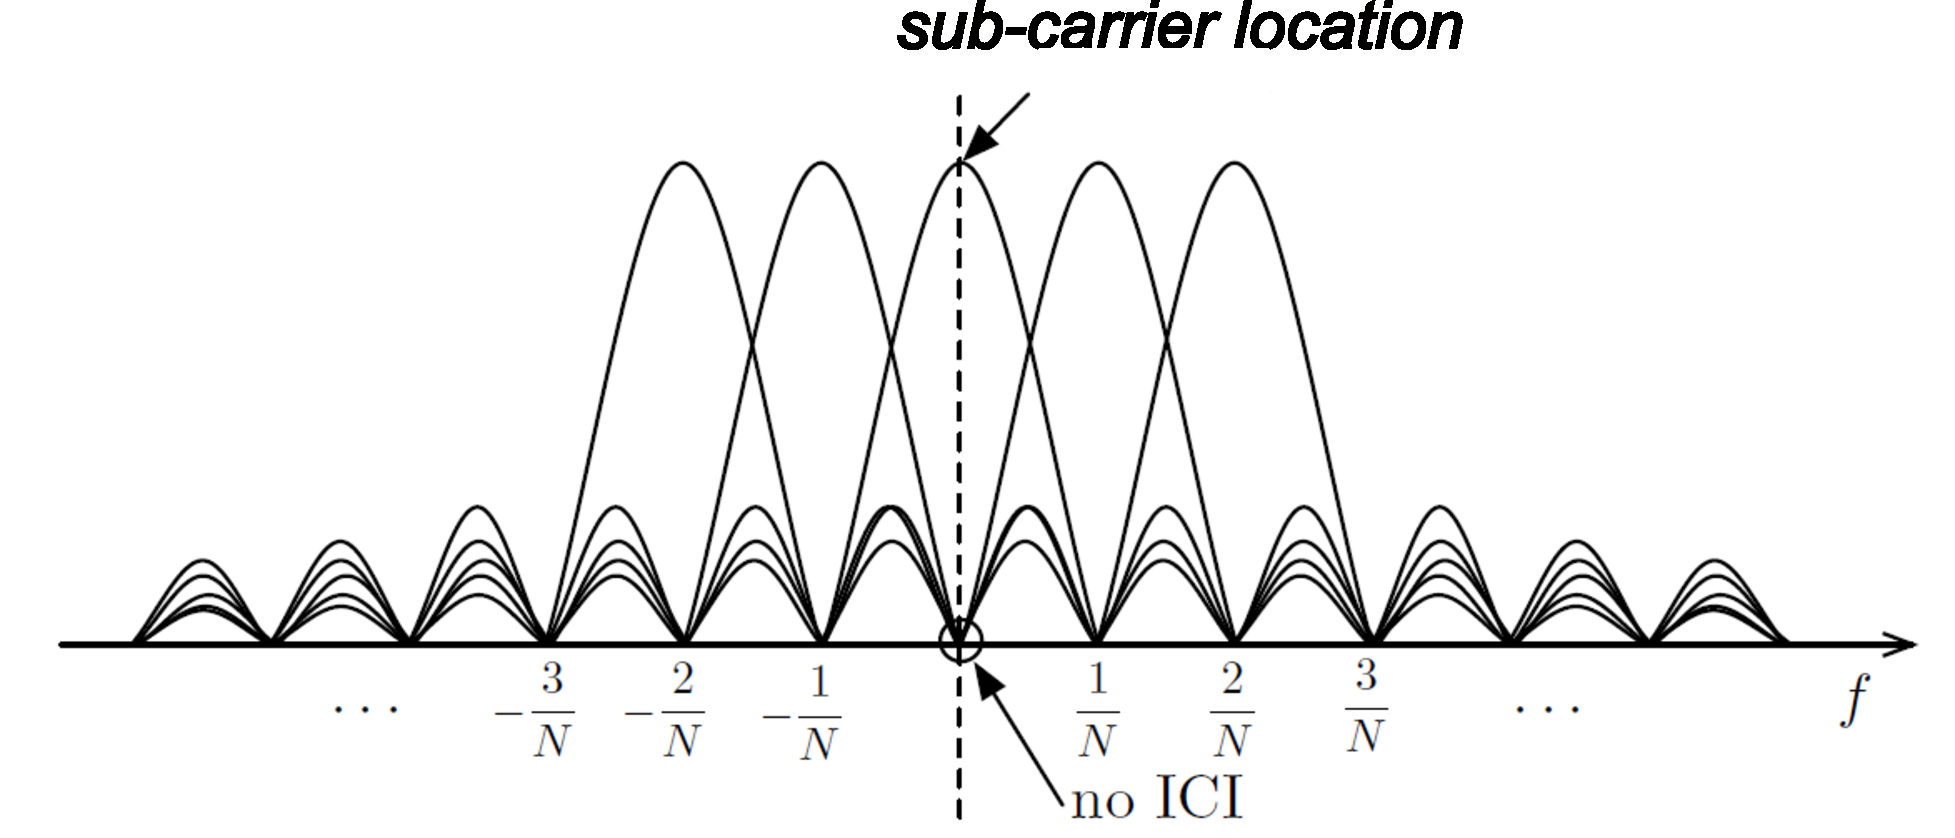
\includegraphics [width=0.8\columnwidth] {Figures/OFDM-subcarrier.pdf} }
	\caption{The spectrum of subcarriers in OFDM \cite{farhang2008signal}}
	\label{fig:OFDM-subcarrier}
\end{figure}

An OFDM symbol signal can be expressed at baseband by a sum of modulated complex exponentials as:

\begin{eqnarray}
\label{equ:OFDMsignal}
s(t) = \sum_{k=0}^{N-1} X_k e^{i2\pi\Delta ft},
\end{eqnarray}
where $X_{k}$ represents a data modulated symbol such as a BPSK, QPSK, or QAM symbol, and is a complex number modulated by the $kth$ subcarrier of $N$ subcarriers and $\Delta f$ is the subcarrier spacing. 
Sampling this OFDM symbol signal with sampling period of $T_S$ is expressed as:

\begin{eqnarray}
\label{equ:sampledOFDMsignal}
s(nT_S) = \sum_{k=0}^{N-1} X_k e^{i2\pi\Delta fnT_S},
\end{eqnarray}
A sample of the OFDM signal is equivalent to an inverse N-point discrete Fourier transform (IDFT), taking $X_{k}$ as a discrete point in the frequency domain. 
Inversely, the sampled OFDM symbol signal can be demodulated using the discrete Fourier transform (DFT). The OFDM modulation and demodulation are hence performed by computing the IDFT and DFT, respectively, expressed as:

\begin{eqnarray}
\label{equ:sampledOFDMsignal}
s[n] = \frac{1}{N}\sum_{k=0}^{N-1} X[k] e^{i2\pi\frac{k}{N}n},
\end{eqnarray} 
\begin{eqnarray}
\label{equ:sampledOFDMsignal}
X[k] = \sum_{n=0}^{N-1} s[n] e^{-i2\pi\frac{k}{N}n},
\end{eqnarray} 

In order to achieve efficient computation, The inverse Fast Fourier Transform (IFFT) and Fast Fourier Transform (FFT) are implemented in an OFDM system to modulate and demodulate the signal instead of the IDFT and DFT, respectively. These optimised algorithms generally rely on the number of points, and hence carriers, being a power of 2.

%---------------------------------------------------------------------------------
\subsection{Cyclic Prefix}
%---------------------------------------------------------------------------------

When transmitting OFDM symbols over a delay-dispersive multi-path channel, the received signal is the linear convolution of the transmitted symbol with the channel impulse
response (CIR) 

\begin{eqnarray}
\label{equ:sampledOFDMsignal}
y[n] = h*s[n],
\end{eqnarray} 

where $h$, assuming it has a length of $L$, denotes the equivalent impulse response of the channel. and $*$ is the convolution operation. 
The received symbols $y[n]$ are the result of convolution between CIR $h$ and transmitted symbols $s[n]$ which has a length of $N$.
So,  $y[n]$ has a length of $N+L-1$.
In addition, the received signal is obtained by concatenating the received OFDM symbols. 
Because the received symbols, having a length of $N+L-1$, are overlapped with the adjacent received symbols, adding the overlap of adjacent received symbols leads to the introduction of the Inter Symbol Interference (ISI) in the received signal shown in Fig.~\ref{fig:CIR-noCP}.


\begin{figure}
	\centerline{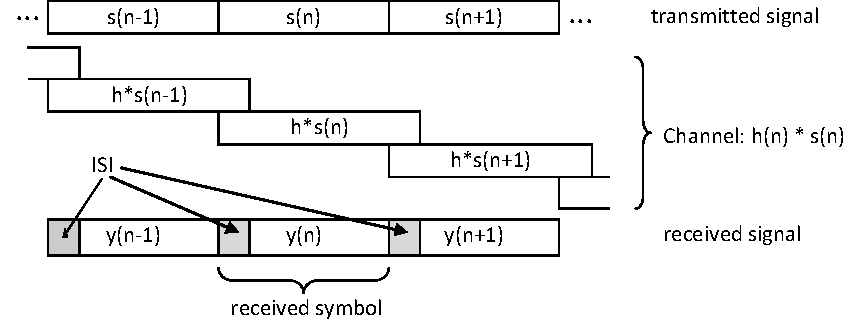
\includegraphics [width=0.8\columnwidth] {Figures/CIR_noCP.pdf} }
	\caption{OFDM transmission without cyclic prefix results ISI among adjacent symbol}
	\label{fig:CIR-noCP}
\end{figure}

In order to avoid ISI, a guard interval (or cyclic prefix), having a length of $L_{CP}$, has to be added before each OFDM symbol as demonstrated in Fig.~\ref{fig:CIR-CP}. 
If the length of CIR, $L$, is smaller than that of the guard interval, $L_{CP}$, adding the overlap of adjacent received symbols will not interfere with the succeeding received OFDM symbol. 
The ISI is hence missing in the received symbol.  
The guard interval, adopted in standards, can be commonly performed by a copy of the last $L_{CP}$ samples of the symbol as shown in Fig.~\ref{fig:CP}, that is called a cyclic prefix (CP)

\begin{figure}
	\centerline{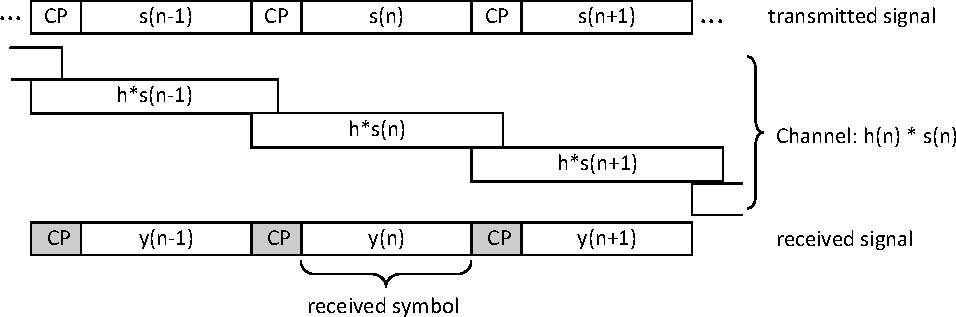
\includegraphics [width=0.8\columnwidth] {Figures/CIR_CP.pdf} }
	\caption{OFDM transmission with cyclic prefix avoids ISI among adjacent symbol}
	\label{fig:CIR-CP}
\end{figure}

\begin{figure}
	\centerline{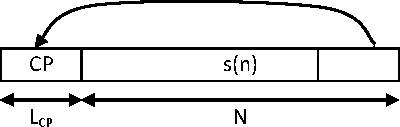
\includegraphics [width=0.8\columnwidth] {Figures/CP.pdf} }
	\caption{Inserting Cyclic Prefix in the OFDM symbol}
	\label{fig:CP}
\end{figure}

In addition, the use of CP also guarantees the orthogonality of subcarriers avoiding the ICI. Performing DFT operation and a single-tap equalizer per subcarrier allows recovery of the transmitted symbols \cite{farhang2008signal}. 

%---------------------------------------------------------------------------------
\subsection{OFDM-based system}
%---------------------------------------------------------------------------------
In the above section, the OFDM modulation technique was presented, and inserting CP was introduced to improve the performance of OFDM in multi path channel. 
A OFDM-based system model can be equivalently considered as shown in Fig.~\ref{fig:OFDM-model}.

\begin{figure}
	\centerline{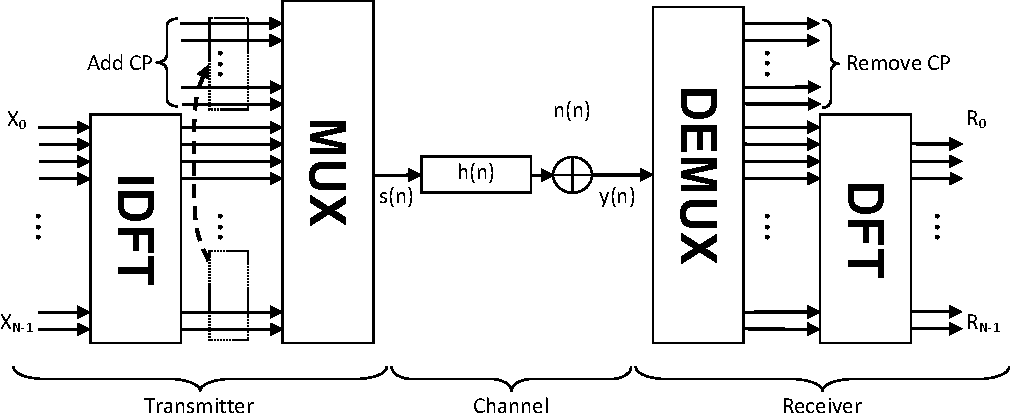
\includegraphics [width=0.8\columnwidth] {Figures/OFDM-model.pdf} }
	\caption{the OFDM system model}
	\label{fig:OFDM-model}
\end{figure}

In the transmitter, the data modulated symbols $X[n]$ are grouped in a blocks of $N$ sub-carrier symbols known as an OFDM symbol, expressed by a vector $X[n]=(X[1], X[2], ..., X[n])^T$. 
Next, the OFDM symbol signal in the time domain is modulated by performing IDFT on each OFDM symbol, and a cyclic prefix of length $L_{CP}$ is inserted at the begin of OFDM signal. 
So, the complex signal of $m$, the OFDM-symbol in baseband discrete time, can be expressed as
\begin{eqnarray}
\label{equ:OFDMsymbol}
s_{m}[n] = \frac{1}{N} \sum_{k=0}^{N-1}X[k]e^{i2\pi k\frac{n-L_{CP}}{N}},
\end{eqnarray} 

where $n$ is the discrete time index, $m$ denotes the index of the OFDM symbol. 
The complete transmitted signal in the discrete time domain, $s[n]$, is given by the concatenation of all OFDM symbols, $s_{m}[n]$,

\begin{eqnarray}
\label{equ:OFDMsignal}
s[n] =  \sum_{m=0}^{\infty} s_{m}[n-m(N+L_{CP})],
\end{eqnarray} 

When transmitting OFDM signals over a multi-path channel, the received signal is obtained through the linear convolution of the transmitted symbol with CIR $h[i]$ and adding additive white Gaussian noise (AWGN) $n$. 
Assuming that the synchronisation between the transmitter and receiver are perfectly achieved, the channel fading is slow enough to consider as a time invariant channel during one OFDM symbol interval, and the length of cyclic prefix is longer than that of CIR ($h[i] = 0$ for $i < 0 i > L_{CP}-1$), 

\begin{eqnarray}
\label{equ:OFDMchannelsignal}
y[n] =  \sum_{i=0}^{L_{CP}-1} h[i]s[n-i] + n[n],
\end{eqnarray} 

In the receiver, the incoming samples $y[n]$ are synchronously  grouped into block of OFDM symbols and then the cyclic prefix in each OFDM symbol is removed. 
The received symbols can be expressed in a vector $y_{m} = (y_{1}, y_{2}, . . . )$ , with $y_{m}[n]=y[m(Nc+Ncp)+Ncp +n]$.
The received data symbols associated with $m^{th}$ OFDM symbol $R_{m}[n]$ are retrieved by performing a $N$-point DFT:

\begin{eqnarray}
\label{equ:receiveOFDMsymbol}
R_{m}[n] =  \sum_{n=0}^{N-1} y_{m}[n]e^{-i2\pi \frac{nk}{N}},
\end{eqnarray} 

\begin{figure}
	\centerline{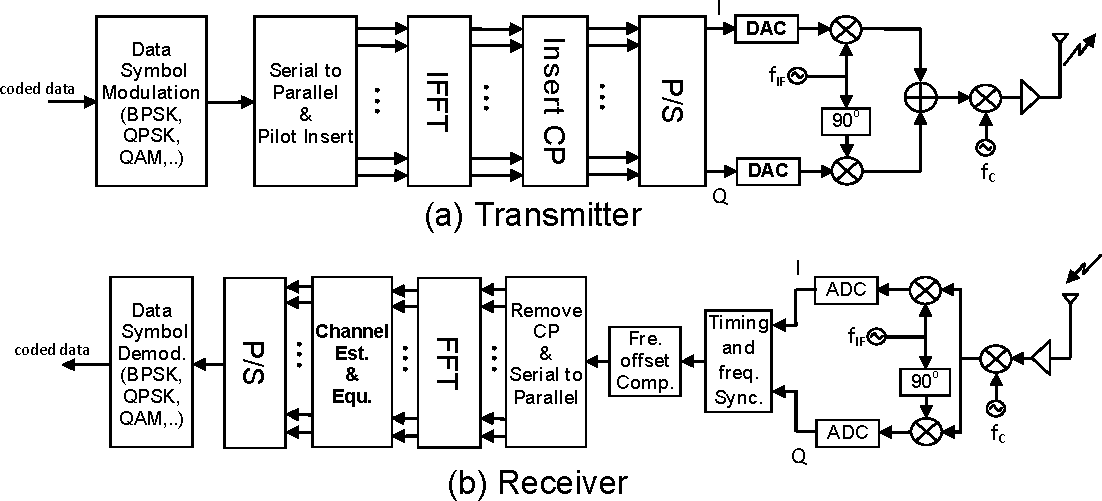
\includegraphics [width=0.8\columnwidth] {Figures/OFDM-block.pdf} }
	\caption{The block diagram of OFDM-based RF systems}
	\label{fig:OFDM-block}
\end{figure}

Fig.~\ref{fig:OFDM-block} presents the common block diagram of an OFDM-based RF system.
OFDM is perform in the baseband, IFFT and FFT blocks are used to compute IDFT and DFT for OFDM modulation and demodulation, respectively.
In the transceiver, the channel coded data from higher abstracted layers is modulated to data symbols (BPSK, QPSK, QAM, ...). The data symbols are then grouped together with the pilots to form $N$ FFT points in parallel.
After performing IFFT, the CP is inserted, and then the OFDM samples are serialised and split in to in-phase (I) and quadrature (Q) channels corresponding to the real and imaginary parts of  the OFDM sample. 
The digital to analogue converted signals of I and Q channels are modulated by an intermediate frequency, $f_{IF}$, then the signal is up-converted to high frequency by an RF carrier, $f_{C}$. 
Before transmitting, the signal should be amplified by an low noise amplifier (LNA).

In the receiver, after down-converting and IQ demodulation, the signal is sampled. The samples are formed from I and Q channels corresponding to the real and imaginary parts of the OFDM sample.
The timing and frequency synchronisation blocks detect the frame, recover timing of the frame and estimate the frequency offset. 
The received samples are then compensated by estimated frequency offset in the discrete time domain. 
After demodulating an OFDM symbol using FFT, estimating the channel and then channel equalisation as well as phase error compensation are performed to improve performance.
The block of parallel samples in an OFDM symbol is serialised to data symbol sequences that are then demodulated, and coded data is sent to higher abstracted layers to decode.

%---------------------------------------------------------------------------------
\subsection{Evaluating OFDM}
%---------------------------------------------------------------------------------

The main advantages of OFDM are its spectrally efficient usage and robustness against multi path propagation.
This makes OFDM suitable for high performance wireless applications. 
OFDM uses multiple sub-carriers which are overlapped with other subcarriers in the frequency domain, resulting in greater spectral efficiency than FDM. 
Performing OFDM is equivalent to splitting a data stream into several parallel low-rate streams before transmission.
This makes the OFDM signal more robust against fading when transmitted through the channel. 
Thanks to the cyclic prefix, the ISI and ICI caused by the multi-path channel can be eliminated. 
The CP creates a guard period for an OFDM symbol, which should be longer than the CIR to ensure no ISI.
Repeating samples of the OFDM symbol in a guard period, the CP helps to maintain the orthogonality of subcarriers avoiding the ICI. 
Thus, performing the DFT and a single-tap equalizer per subcarrier allows recovery of the transmitted symbols.

On the other hand, OFDM has some disadvantages. 
Firstly, an OFDM signal is the sum of multiple modulated sub-carriers, and thus suffers a high peak-to-average power ratio (PAPR). 
This results in demand on high power and wide range linearity in amplifiers increasing the cost of OFDM-based systems.
Secondly, the usage of guard period reduces bandwidth efficiency of OFDM.
Last but not least, OFDM performance is sensitive to receiver synchronisation. Frequency offset causes inter-subcarrier interference and errors in timing synchronisation can lead to inter-symbol interference.
Much effort is needed to improve the accuracy of both frequency and time synchronizers for OFDM.

%-------------------------------------------------------------------------------------------------------------------------------------------------------------------------------------------------------------------------------------------------------------
\section{Multiple Standard Cognitive Radios}
%-------------------------------------------------------------------------------------------------------------------------------------------------------------------------------------------------------------------------------------------------------------

The spectral resource demands of wireless telecommunication systems continues to increase. %Practically, radio spectrum is not fully usage regarding to its capacity by regulatory and license processes for spectral allocation.
Cognitive Radios (CRs), that have ability to adapte to channel conditions, ensuring effective spectrum usage, are an important technology for achieving this. 
They are designed to transmit in currently unused spectrum without causing harmful interference to primary users (PUs) or incumbent users (IUs).
Apart from the critical issues of spectrum sensing and band allocation, the lower priority of secondary users (SUs) raises a challenge in terms of transmission capability and quality of service in cognitive radios. 
When the spectrum allowed for a CR system is fully occupied by PUs and IUs, the transmission of CRs can be blocked. 
Multiple Standard Cognitive Radios (MSCRs) are able to operate in multiple frequency bands with different specified standards.
MSCRs are hence a more flexible generalisation of CRs as they can operate across different bands and standards.

%Most practical CRs are built using powerful general purpose processors to achieve flexibility through software, but they can still fail to offer the computational throughput required for advanced modulation and coding techniques and they often have high power consumption.
%GNU Radio~\cite{gnuradio} has been a widely used platform in academia. 
%It is a software application that runs on a computer or an embedded ARM processor platform, e.g. on the Ettus USRP E100. 
%Computational limitations mean that while it has been successful for investigating CR ideas, it is not feasible for implementing advanced embedded radios using complex algorithms.
%Other software based frameworks like Iris~\cite{Sutton2010}, have some limited support for FPGAs but suffer from poor bandwidth between software and hardware.

%In an application area with fast moving standards and requiring support for multiple standards, custom ASIC implementation is prohibitive.
%Delorme et al.~\cite{Delorme2008} presented a heterogeneous reconfigurable hardware platform for Cognitive Radio. 
%It can adapt its hardware structure to support standards like GSM, UMTS, wireless LAN. 
%Most processing components run as embedded software on the nodes in a network on chip, while the channel coder and the mapping of the RX chain are implemented inside an FPGA. 
%Partial reconfiguration is used to switch the channel coder from one context to an another depending on SNR. 
%A processor manages data movement between the different processors, the ASIC, and the FPGA. The need for a large data buffer and inefficient data transfer mechanisms lead to increased power consumption and reduced throughput.
%There are few studies on FPGA based platforms for radio implementation. 
%KUAR~\cite{Minden2007} is a mature radio platform built around a fully-featured Pentium PC with a Xilinx Virtex II FPGA. 
%The baseband processing is accelerated on FPGA and only limited for NC-OFDM signal based on the IEEE 802.16 standard.
%Projects at Virginia Tech~\cite{athanaswires} have shown dynamically assembled radio structures on FPGAs, where the target radio system is defined at a high-level with datapaths connecting relatively large functional modules. 
%The modules are wrapped, and each of them consists of a PR module with complied partial bit-streams stored in dynamic library. 
%Using PR eliminates the need for run time compilation, but affording flexibility . 
%A flexible radio controller can insert and remove compiled modules to adapt to current conditions.

Multi-carrier modulation techniques offer an ideal opportunity for such systems due to their regularity and parameterisation. OFDM and Filter Bank Multi Carrier (FBMC) are two types of multi-carrier modulations. OFDM modulation has been the dominant technique adopted for many standards and has been investigated in terms of spectral sensing and carrier allocation for CRs. 
Furthermore, OFDM system implementation is simple, low cost, and can be effectively parameterised in comparison to FBMC systems. OFDM is a suitable candidate for a MSCR system. The advantages of coupling OFDM modulation with an FPGA platform are investigated for the feasibility of implementing the proposed MSCR system. 
The flexibility requirement of a MSCR is to support existing standards like 802.11, 802.16, and 802.22, as well as supporting future OFDM-based standards.

A feasible OFDM-based MSCR requires the ability to switch baseband processing from one standard to another. This means that the system needs to rapidly adapt its functionality to perform variable numbers of FFT/IFFT operations, insert CP of configurable length, and handle differend pilot vectors as well as different preambles. The hardware implementation of an OFDM-based MSCR can be based on the original architecture of an OFDM system illustrated in Fig.~\ref{fig:OFDM-block}. However, each sub-module of the system needs to be designed to perform with all parameters of the supported standards. This results in significantly increasing system complexity as well as reconfiguration time.   

%One way this can be done is for separate implementations of each standard to be implemented as partial bitstreams which are swapped at runtime. However, a large monolithic bitstream requires a longer reconfiguration time. Our proposed approach uses a finer granularity. Each module in the processing chain is investigated and commonalities across standards are analysed. For modules requiring only minor modifications, parameterised versions are created. For those that require significant changes, PR can be used on a per-module level. As a result, when switching from one standard to another, only part of the FPGA needs to be reconfigured.

Beside the challenge of long configuration time for MSCR, there are two key challenges of the baseband related to the synchronizer and spectral shaper. OFDM systems typically tolerate a small carrier frequency offset (CFO) leading to strict constraints on the design of the RF front-end. In an MSCR system, the RF front-end should access a wide range of frequencies depending on the standard in operation. Such a precise and yet wide ranging frequency requirement makes the RF front-end design difficult if not impossible or require very expensive components.
CRs also demand small spectral leakage for both in-band and out-of-band transmitted signals to avoid causing harmful interference to primary users, while OFDM signals have intrinsically large side lobes leading to a potentially large degree of spectral leakage. 
Flexibility in the baseband can allow a frequency guard extending technique to achieve spectral leakage requirements.

The interface to the higher layer processing is another important factor. Many hardware radio platforms are extremely difficult to design for or to modify. Hence, only hardware experts can use them. While detailed optimisation of low level blocks is important, providing a general interface for implementing higher layer processing is also important. This ensures that radio experts may use the system to investigate cognitive radio techniques without the need for specific advanced low-level FPGA expertise.


%-------------------------------------------------------------------------------------------------------------------------------------------------------------------------------------------------------------------------------------------------------------
\section{OFDM Synchronisation}
%-------------------------------------------------------------------------------------------------------------------------------------------------------------------------------------------------------------------------------------------------------------

OFDM performance is sensitive to receiver synchronisation. 
Frequency offset causes inter-subcarrier interference, and errors in timing synchronisation can lead to intersymbol interference. 
Therefore, synchronisation is critical for good performance in OFDM systems. 
There are two main errors implicit in synchronisation: sample clock timing offsets and carrier frequency offsets.
In order to obtain good synchronisation performance, timing offsets and frequency offsets must be studied in terms of their cause and effect on the degradation of OFDM received data symbols.
Additionally, there are issues of common phase error (CPE), generated from clock jitter and phase noise, that causes a random rotation of the entire signal constellation.
This must also be taken into account and compensated for in order to achieve good performance.

%---------------------------------------------------------------------------------
\subsection{Timing Offsets}
%---------------------------------------------------------------------------------

When sampling a signal at the receiver, the different times of sampling between samples in the receiver and transmitter are referred as timing error.
In a single carrier system, the symbol clock in the transmitter can be recovered at the receiver using a phase-lock loop (PLL) \cite{farhang2008signal}. 
This can correct a timing error in the receiver relatively easily.

In OFDM, however, timing errors can be considered in two categories: fractional and integer. 
Fractional timing error, that is errors that are smaller than one sample period, are caused by different phases between the sampling clock of the analogue to digital converter (ADC) in the receiver and the phase of the transmitted signal, while integer timing error is that which is greater than one sample period, causing index shifting, or offset, in the sample sequence.

The timing error in the time domain is equivalent to a phase rotation in the frequency domain expressed in Equ. (\ref{equ:timingoffset}),

\begin{eqnarray}
\label{equ:timingoffset}
               s (t - \tau )   \Leftrightarrow  e^{-i2\pi f\tau} R(f),
\end{eqnarray}	
where $\tau$ denotes timing error resulting in a phase shift of $e^{-i2\pi f\tau}$. 
$s(t)$ is the received signal in the time domain, and $R(f)$ is the spectrum of $s(t)$ in the frequency domain.
The phase shift is proportional to both time errors and the frequency of carriers.
In the case of multi-carriers with increasing frequency, the phase shift is increased according to the carriers leading to the phase rotation of subcarriers.
Carrier rotations caused by fractional timing error $\Delta t$ like that caused by fading can be estimated by a channel estimator and compensated for after performing the DFT,
\begin{eqnarray}
\label{equ:rotationcompensation}
               \widehat{R[n]} = R[n] e^{\frac{i2\pi n \Delta  t}{N}},
\end{eqnarray}
where $R[n]$, $\widehat{R[n]}$ denotes received data symbols before and after compensation, respectively. $\Delta t$ is estimated phase rotation, and N is the number of sub-carriers.

Moreover, the received samples in the receiver are synchronously grouped into blocks of OFDM symbols.
Integer timing errors lead to a symbol timing offset (STO) referring to the difference between correct sample index and the actual sample index of received samples that causes a misaligned window for DFT demodulation in the receiver.
If the timing offset is late, the samples of the following symbol are used for the current symbol, resulting in ISI and hence degrading the performance of the OFDM system. The effect of ISI caused by later timing offsets on the OFDM received symbol is illustrated in Fig.~\ref{fig:Timingoffsetconstellation}(a) and Fig.~\ref{fig:Timingoffsetconstellation}(c).
If the timing offset is early, some samples in the CP of the current symbol are used to calculate the DFT, leading to sub-carrier rotation expressed in Equ.\ref{equ:timingoffset} in the frequency domain.  
The effect of sub-carrier rotation caused by earlier timing offsets on the OFDM received symbol is illustrated in Fig.~\ref{fig:Timingoffsetconstellation}(b) and Fig.~\ref{fig:Timingoffsetconstellation}(d).

\begin{eqnarray}
\label{equ:rotationcompensation}
              s[n - \mathit{t_{off}}]  \Leftrightarrow R[n] e^{\frac{i2\pi n \mathit{t_{off}}}{N}},
\end{eqnarray}
where $s[n]$, $R[n]$ denotes received data symbols in the timing domain and the frequency domain, respectively. $\mathit{t_{off}}$ is a timing offset, and N is the number of sub-carriers.

\begin{figure}
	\centerline{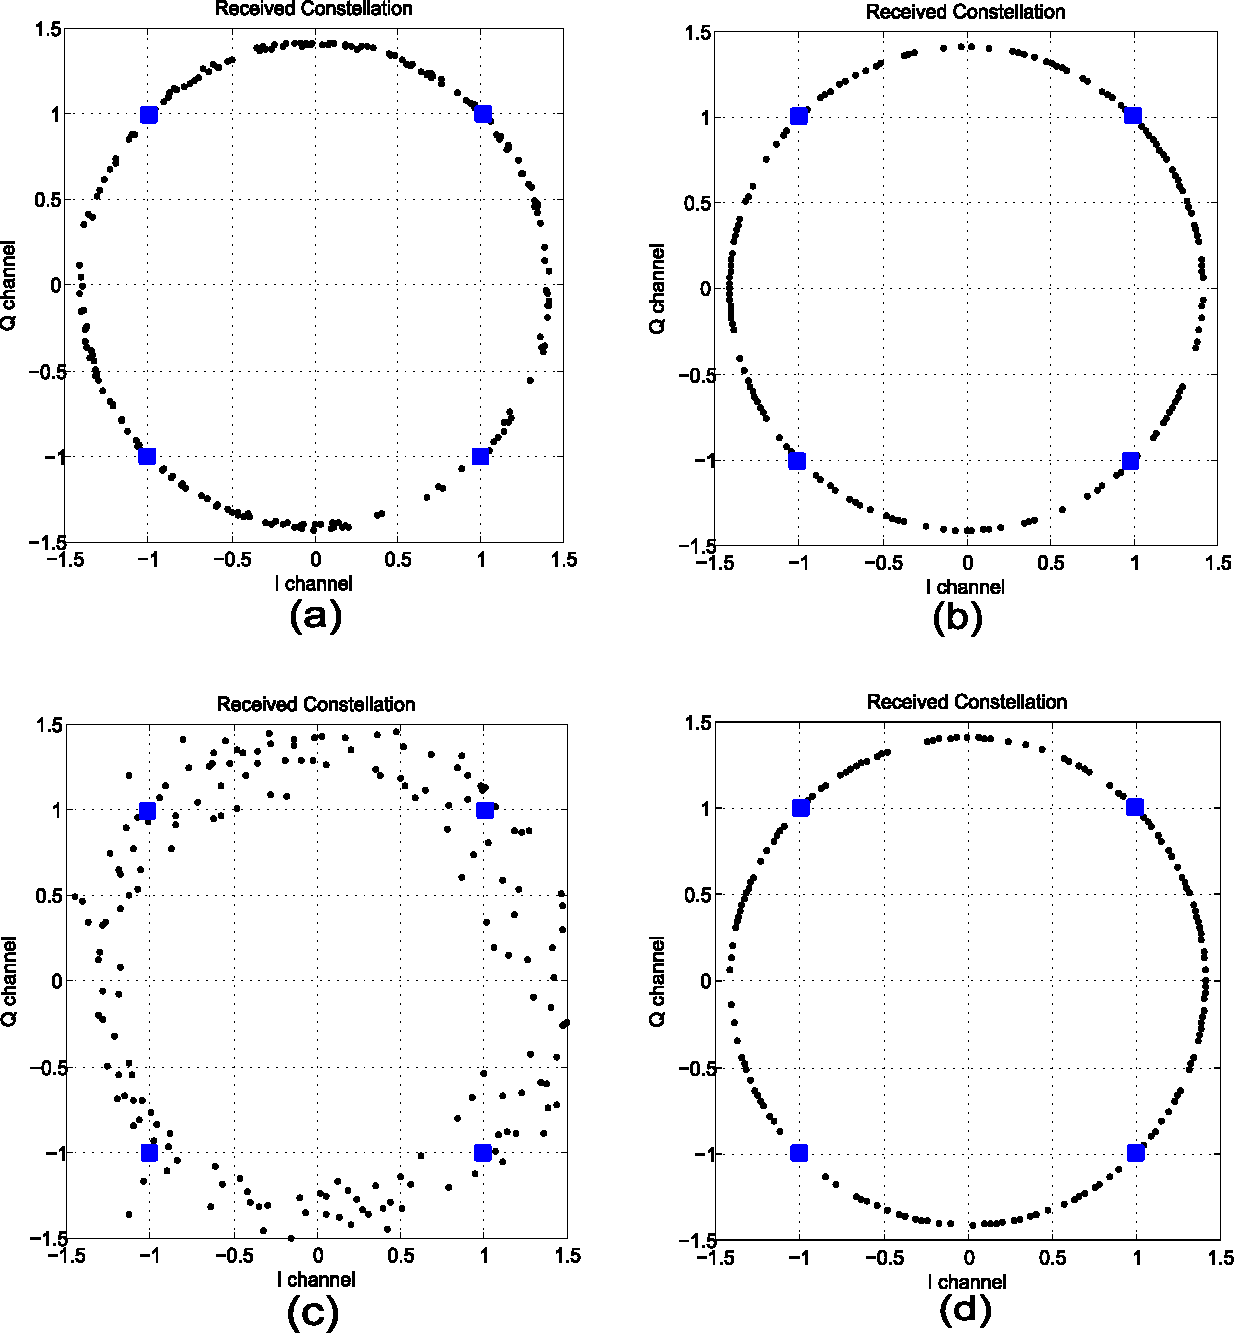
\includegraphics [width=0.8\columnwidth] {Figures/timeoff.pdf} }
	\caption{OFDM received symbol with timing offets of -1, 1, -5 and 5 in a, b, c, d, respectively.}
	\label{fig:Timingoffsetconstellation}
\end{figure}

Fig.~\ref{fig:Timingoffsetconstellation} illustrates the effect of timing offset on a single 256 subcarrier OFDM symbol utilizing QPSK subcarriers (based on the IEEE~802.16).
As can be seen, the earlier timing, for instance timing offsets of 1 and 5, shown respectively in Figs.~\ref{fig:Timingoffsetconstellation}(b) and~\ref{fig:Timingoffsetconstellation}(d), cause a carriers rotation similar to that of fractional timing errors, and fading that can be estimated by a channel estimator.
However, the later timing, for instance timing offsets of 1 and 5, as shown in Figs.~\ref{fig:Timingoffsetconstellation}(a) and~\ref{fig:Timingoffsetconstellation}(c), lead to ISI that prevents the OFDM constellation from being recovered. 
Therefore, timing synchronisation is required to correct the timing offset, and avoid ISI.

%---------------------------------------------------------------------------------
\subsection{Frequency Offset}
%---------------------------------------------------------------------------------

CFO refers to a difference in frequency between the receiver clock with respect to the `correct' frequency of carriers in a transmitted OFDM symbol. 
CFO is introduced by an imperfect clock in the RF front-end part, as well as by frequency variation caused by the Doppler effect when a signal is transmitted through a frequency selective channel. 
This leads to the misalignment of sampling in sub-carriers in the frequency domain that causes a loss of orthogonaltity because at the point of frequency offeset in the sub-carrier, the other sub-carriers are not null as expected (shown in Fig.~\ref{fig:OFDM-subcarrier-freoff}).


\begin{figure}
	\centerline{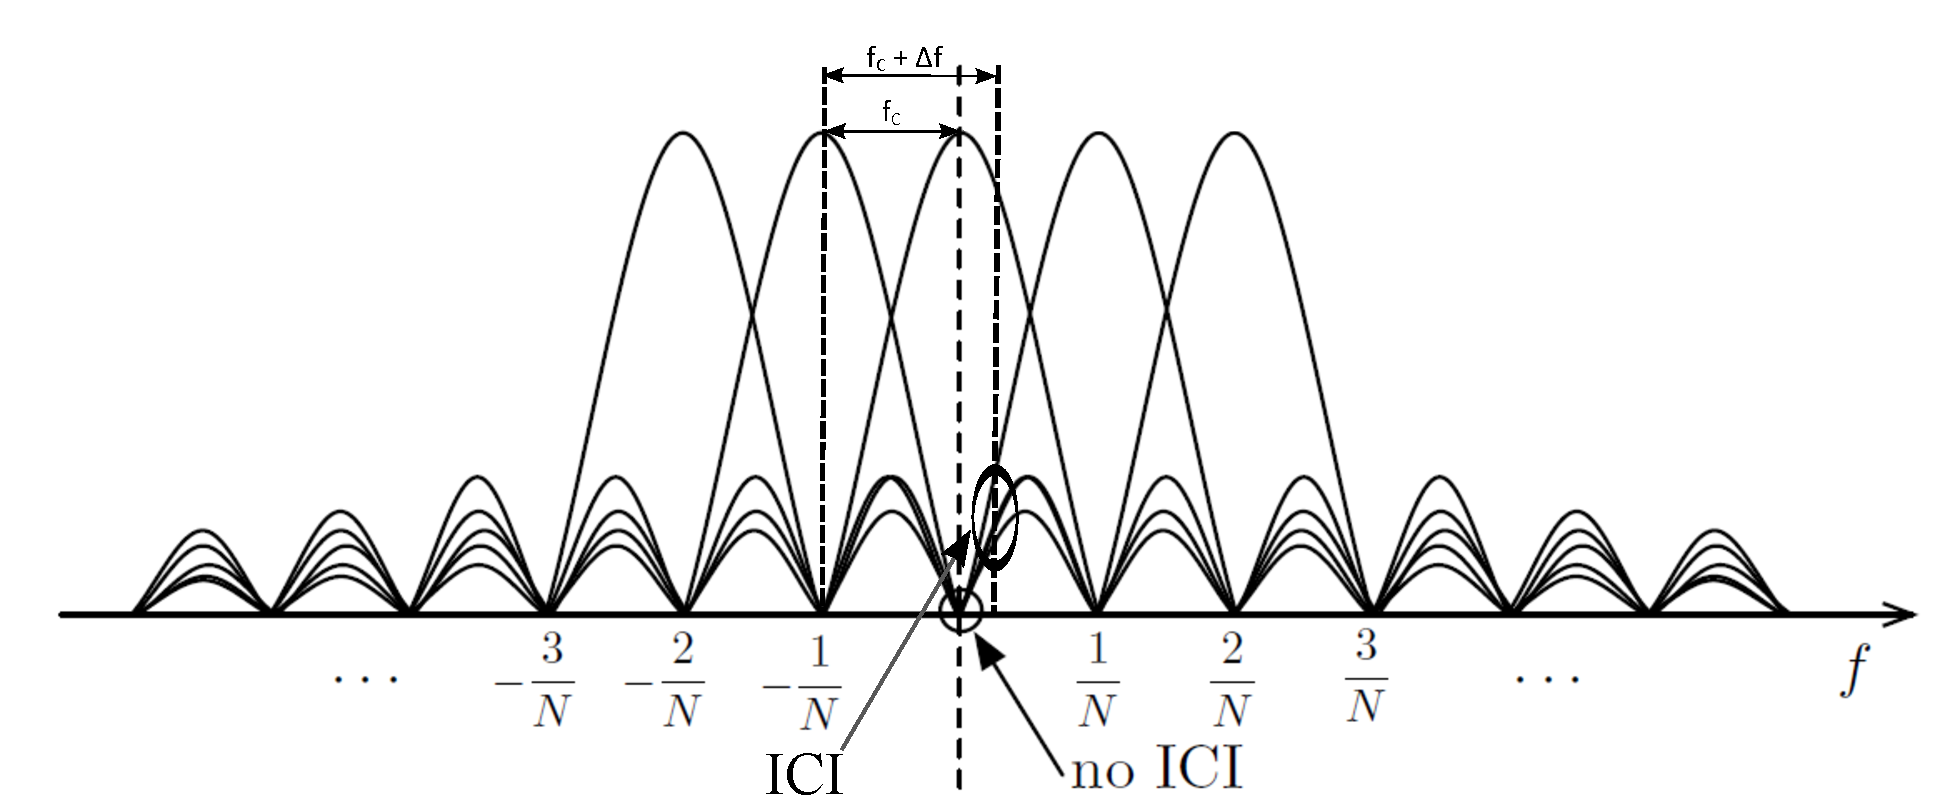
\includegraphics [width=0.8\columnwidth] {Figures/OFDM-subcarrier-freoff.pdf} }
	\caption{Inter carrier interference (ICI) caused by frequency ofsset $\Delta f$.}
	\label{fig:OFDM-subcarrier-freoff}
\end{figure}

With no frequency offset, the frequency bin of the DFT will be sampled at the value at the peak of each subcarrier, $sinc(x)$ pulse, and other adjacent pulses are null at this point. 
However, if frequency offset is introduced, the frequency bin of the DFT will sum the energy from other sub-carriers. 
This means that the adjacent subcarrier introduces an interference component resulting in ICI. 

As can be seen, the adjacent subcarrier introduces an interference component that is about half the amplitude of the subcarrier of interest. 
All other subcarriers introduce an interference component of much lower amplitude. 
This is known as a loss of orthogonality, and must be compensated for in order to properly demodulate the OFDM symbol.
The effect of CFO can be easily considered in the time domain by taking an inverse Fourier transform expressed as follows:

\begin{eqnarray}
\label{equ:}
             R(f - \Delta f) \Leftrightarrow  e^{i2\pi \Delta ft} s(t),
\end{eqnarray}	

In the discrete time domain, the signal sample sequence can be expressed: 
\begin{eqnarray}
\label{equ:}
            s[n]' = s[n] e^{\frac{− i2\pi \Delta fn}{N}},
\end{eqnarray}
where $s[n]'$ and $s[n]$ are the frequency offset samples and the original samples, respectively.
$\Delta f$ denotes the frequency offset, and $N$ is the number of subcarriers. 

The effect of frequency offset is shown in Fig.~\ref{fig:freoff_1sym}. Each plot illutrates the constellation of QPSK symbols demodulated from one 256 sub-carrier OFDM symbol based on the IEEE~802.16 standard.

\begin{figure}
	\centerline{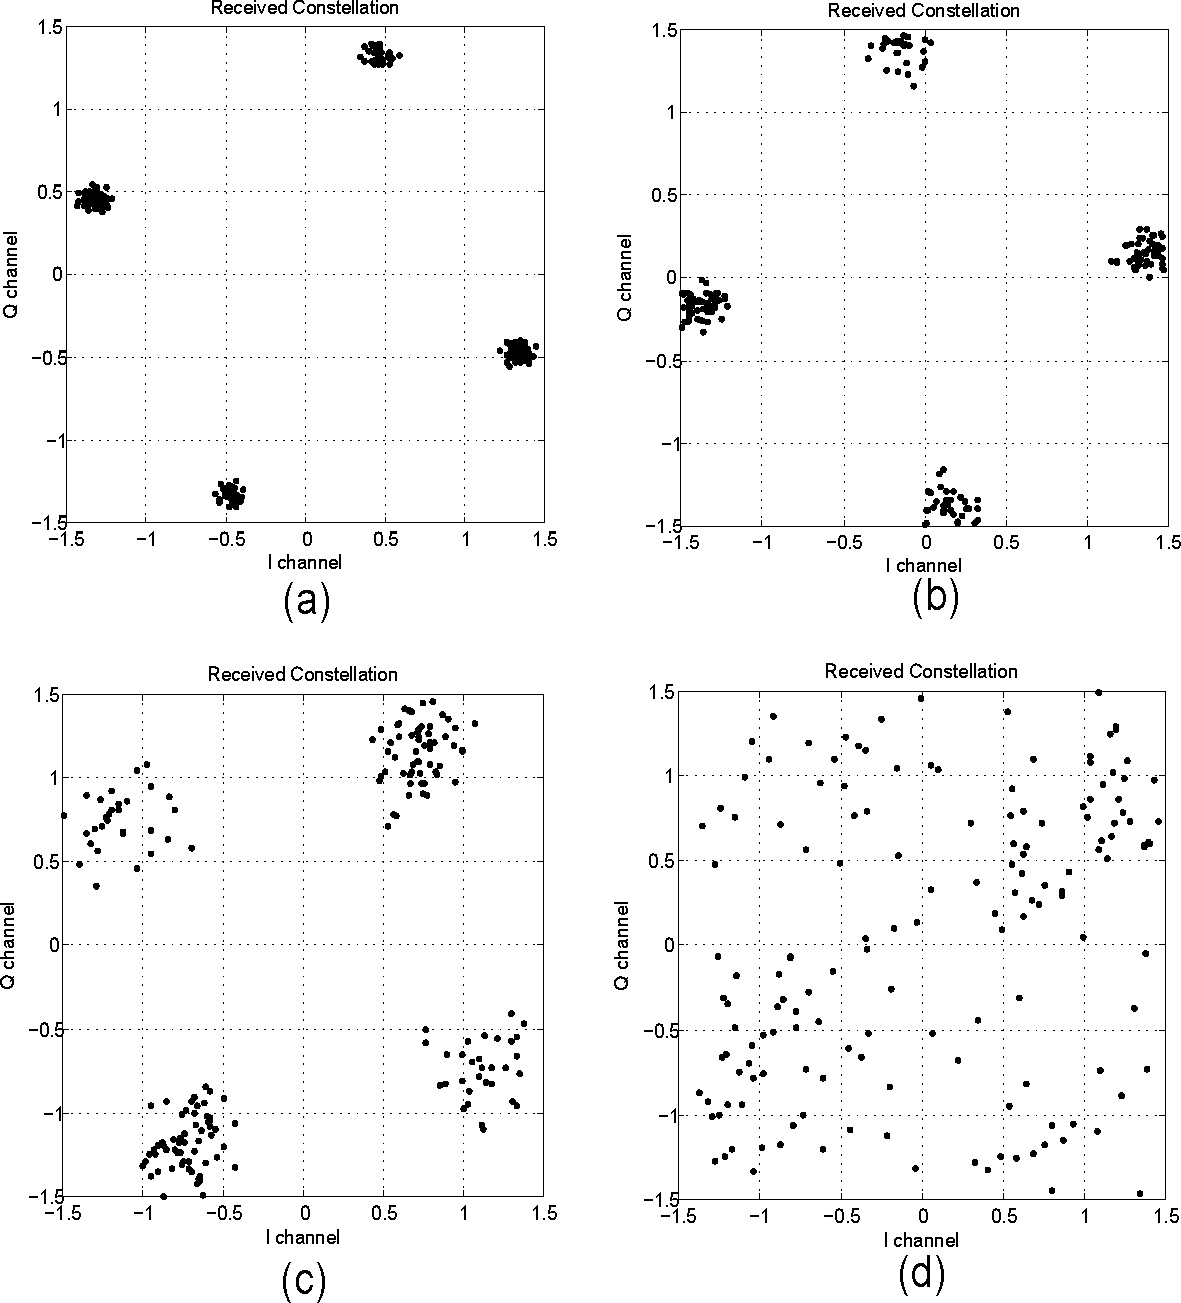
\includegraphics [width=0.8\columnwidth] {Figures/freoff_1sym.pdf} }
	\caption{The constellations of OFDM received symbol with frequency offets of 0.025, 0.5, 0.1 and 0.25 sub-carries spacing in a, b, c, d, respectively.}
	\label{fig:freoff_1sym}
\end{figure}

As can be seen, OFDM performance is sensitive to even small frequency offsets. 
The effect of CFO causes dispersion, similarly to AWGN, and also phase rotation in the QPSK constellation demodulated from OFDM symbol.
If multiple data symbols are transmitted in a packet, the phase rotation of each OFDM symbol increases, and even small CFO will lead to a large drift of constellation points, shown in Fig.~\ref{fig:freoff_5sym} degrading the performance of demodulation. CFO must be estimated and compensated for, in order to properly demodulate the OFDM symbol.

\begin{figure}
	\centerline{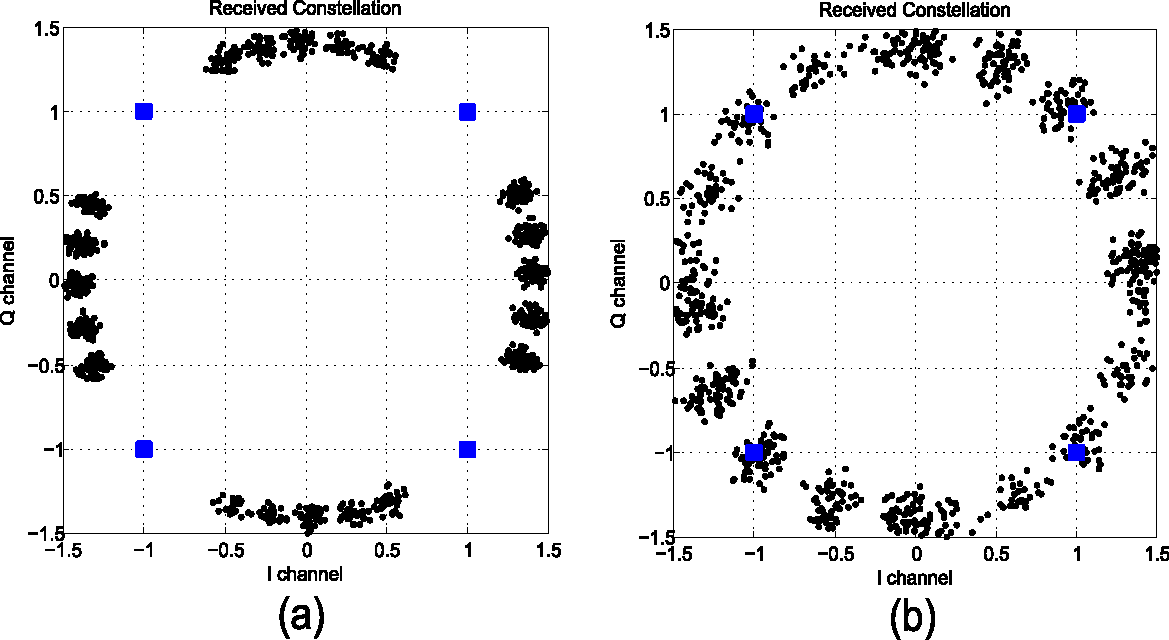
\includegraphics [width=0.8\columnwidth] {Figures/freoff_5sym.pdf} }
	\caption{The constellations of 5 consecutive OFDM received symbols with frequency offets of 0.025 and 0.05 in a, b respectively.}
	\label{fig:freoff_5sym}
\end{figure}

%---------------------------------------------------------------------------------
\subsection{Phase Noise}
%---------------------------------------------------------------------------------

The intrinsic imperfection of the local clock at the RF front-end of a receiver or clock jitter of an ADC may introduce a parasitic phase noise which can affect the performance of baseband data symbols, such as QPSK, QAM, ..., during demodulation.
Phase noise can be considered in two different parts: common phase error and inter-carrier interference \cite{Armada1998}. The effect of phase noise can be expressed in the discrete time domain as:
\begin{eqnarray}
\label{equ:}
            s[n]' = s[n] e^{i\phi[n]},
\end{eqnarray}	
where $s[n]’$ and $s[n]$ are the frequency offset samples and the original samples, respectively.
$\phi[n]$ denotes the phase noise.

If the phase noise is varying more slowly than the OFDM symbol interval, it can be considered a constant phase term added to each sample resulting in CPE \cite{Armada1998}. 
However, if the phase noise is varying much faster than the OFDM interval, different phase noise is added to each sample causing the loss of orthogonality, and thus, intercarrier interference.  
Fig.~\ref{fig:phasenoise} illustrates the effect of phase noise on baseband data symbol demodulation in an OFDM received symbol and 5 consecutive OFDM received symbols.
\begin{figure}
	\centerline{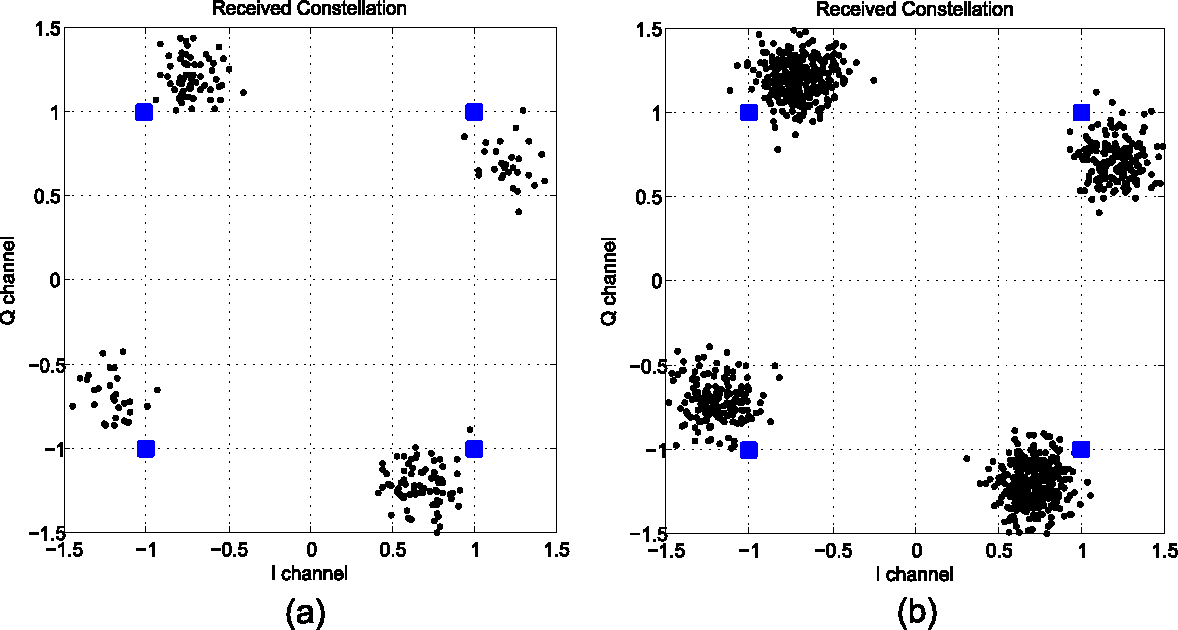
\includegraphics [width=0.8\columnwidth] {Figures/phasenoise.pdf} }
	\caption{The constellations of an OFDM received symbol and 5 consecutive OFDM received symbols with phase noise variance of 0.25 $rad^2$ in (a), (b) respectively.}
	\label{fig:phasenoise}
\end{figure}

As can be seen in Fig.~\ref{fig:phasenoise}, the degradation of OFDM demodulation includes two different phenomena affected by phase noise.
First, the constellations of the data symbol are rotated similarly to the effect of fractional timing error or residual frequency offset.
Second, the constellations of data symbols are dispersed like the effect of AWGN, that causes a loss of orthogonality between the sub-carriers.
However, the difference from the effect of frequency offset will be a constant constellation rotation for all OFDM symbol instead of a different constellation rotation for each symbol in the case of  frequency offset.


%------------------------------------------------------------------------------------------------------------------------------------------------------------------------------------------------------------------------------------------------------------
\section{Shaping OFDM Spectral Leakage}
\label{Ch2:SpecLeak}
%------------------------------------------------------------------------------------------------------------------------------------------------------------------------------------------------------------------------------------------------------------
OFDM modulation techniques have been adopted for many wireless standards as well as enabling technology for cognitive radios.
However, one of their main disadvantages is spectral leakage due to the summation of sinusoidal subcarriers and having been windowed by a rectangular function.
In addition, some recent OFDM-based standards demand very strict requirements on spectral leakage to avoid inter-channel interference.
This raises a significant challenge in how to shape the spectrum of the OFDM signal. 

In 2009, the FCC issued regulatory rules for reusing the television white space (TVWS) spectrum.
IEEE~802.11af was developed under the 802.11 Working Group as a standard that enables a Wi-Fi service in the TVWS spectral regions~\cite{802-11af2013}. 
The scope of the standard is to define amendments to the high throughput 802.11's PHY and MAC layers to meet the requirements for channel access and coexistence in the TVWS regions.
One of the main challenges is the stringent SEM requirements that are mandated by the FCC for these services.. 
The high throughput 802.11 scaled SEM has a large gap between current performance and the required spectral emissions shape for TVWS~\cite{Shellhammer2009}.
For instance, the 802.11 scaled SEM requires an attenuation of 20~dB at the edge of the channel whereas the equivalent this requirement for portable TV band devices (TVBD) is 55~dB.

In 2010, the IEEE defined a standard for PHY and MAC layers~\cite{802-11p2010}, named IEEE~802.11p, for Dedicated Short-Range Communications (DSRC), the wireless channel for new vehicular safety applications through vehicle-to-vehicle (V2V) and Road to Vehicle (RTV) communications.
The PHY in 802.11p is largely inherited from the well-established IEEE~802.11a OFDM PHY, with several changes aimed at improving performance in vehicular environments.
The advantage of building on 802.11a is a potential significant reduction in the cost and development effort necessary to develop the new 802.11p hardware and software.
It also plays an important role in allowing backwards compatibility from 802.11p to 802.11a~\cite{Vandenberghe2011,Fernandez2012}.
Essentially, three changes are made in IEEE~802.11p~\cite{Jiang2008}:
First, 802.11p defines a 10~MHz channel width instead of the 20~MHz used by 802.11a.
This extends the guard interval to address the effects of Doppler spread and inter-symbol interference in a VC channel.
Secondly, 802.11p defines several improvements in receiver adjacent channel rejection performance to reduce the effect of cross channel interference that is especially important in dense vehicle communication channels.
Finally, 802.11p defines four SEMs corresponding to class A to D operations that are specified and issued in FCC~CFR47 Sections 90.377 and 95.1509.
These are more stringent than for current 802.11 radios, in order to improve performance in urban vehicle scenarios.
In addition, 802.11p will operate in the 5.9~GHz DSRC spectrum divided into seven 10~MHz bands. 
This channelization allows the MAC upper layer to perform multi-channel operations \cite{WAVE2010}.
The mechanism allows safety and other applications to occupy separate channels to reduce interference.
The four strict 802.11p SEMs are defined to reduce the effect of ICI between the channels. %, shown in Fig.~\ref{fig:4SEM},
Wu et al. \cite{Wu2013} showed that transmitters on adjacent service channels still cause inter-channel interference (ICI) in the safety channel, even if they satisfy the class C requirement.
Shaping 802.11p  spectral leakage is thus potentially important in helping to eliminate ICI.

Conventionally, there are two methods that can be employed to compress the spectral leakage for OFDM-based system, namely pulse shaping and image spectrum compression. Pulse shaping, recommended in 802.11a, is effective at reducing side lobes. 
Considering an OFDM symbol to have IFFT length and CP length $N$ and $N_{CP}$, respectively, the length of the symbol including its CP is $N_{T} = N + N_{CP}$,
a sample $x[m]$ of the OFDM symbol $(0\leq m \leq N_{T}-1)$ can be expressed in the time domain as,
\begin{equation}
\label{xm}
x[m] = \frac{1}{N}\sum_{k=0}^{N-1} X[k] e^{i2\pi\frac{k}{N}(m-N_{CP})},
\end{equation}
where $X[k]$ denotes the frequency domain representation of the data sub-carriers.
Since OFDM symbol samples are generally transmitted sequentially, this is equivalent to multiplying symbols with a rectangular window function, $p$.
Then the transmitted OFDM samples can be expressed as;
\begin{equation}
\label{equ:xn2}
x[n] = \frac{1}{N}\sum_{l=-\infty}^{\infty} \sum_{k=0}^{N-1} X[k] p[n-l N_{T}] e^{i2\pi\frac{k}{N}(n-N_{CP}-l N_{T})}
\end{equation}
In a conventional OFDM system, the window function, $p(m)$, is rectangular and simply described as;
\begin{equation}
\label{equ:pm}
 p[m] =\begin{cases}1, & m = 0,1, ..., N_{T} \\  0, & otherwise \end{cases}
\end{equation}
In pulse shaping OFDM, the window function, $p[m]$, uses a smooth rather than rectangular pulse resulting in inducing distortion in the subcarriers.
One way to avoid this is to add extending parts, i.e. CP and a cyclic suffix (CS) before and after each conventional OFDM symbol respectively, and to multiply the extended symbol with a smoothing function.
While the CP in conventional OFDM is used as a guard interval, here it is also used for pulse shaping. Pulse shaping extends the  $N_{T}$ length of the OFDM signal by a roll-off factor, $\beta$.
The overhead of extending CS results in spectral loss; overlapping of the CP and CS of consecutive symbols shown in Fig.~\ref{fig:PS} is needed to form a transmitted symbol to reduce this loss, but causes ISI in the overlapped region. Pulse shaping using the overlapping method is effectively equivalent to shortening the OFDM guard interval.
A larger $\beta$ obtains greater compression in spectral leakage but reduces the effective guard interval.
When $\beta N_{T}$ is increased to equal the CP length, the effective guard interval is reduced to zero (no guard interval) to prevent channel-induced ISI.

\begin{figure}[t]
    \centerline{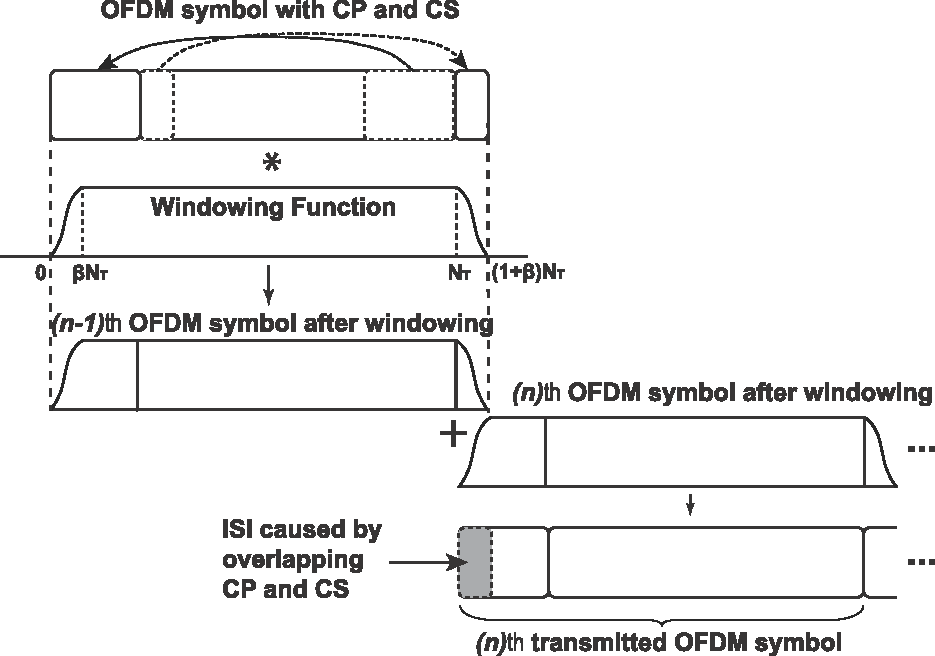
\includegraphics [width=0.9\columnwidth, height=7.5cm] {./Figures/w-ofdm.pdf} }
	\vspace{-2mm}
    \caption{Pulse Shaping operation performed on OFDM symbols.}
    \label{fig:PS}
\end{figure}

Image spectrum compression is implemented as an FIR filter to cancel image spectra.
The Interpolation can be used at baseband to increase sampling frequency, thereby extending baseband bandwidth.
Image spectra are repeats of the original baseband spectrum, present because of interpolation or digital analogue converter (DAC) effects.
On one hand, the narrow band gap between main and adjacent image spectra requires a long impulse response FIR filter.
On the other hand, according to the performance of FIR expressed in (\ref{equ:FIR}), the impulse response of the FIR filter $h$ with length $L_{FIR}$ has a similar effect to the impulse response of the overall channel in terms of inducing ISI.
\begin{equation}
\label{equ:FIR}
y[n] =  \sum_{i=0}^{L_{FIR}-1} h[i]x[n-i] 
\end{equation}

The FIR filter reduces the effective guard interval of OFDM symbols~\cite{farhang2008signal}.
Its design also needs to deal with the tradeoff between the length of filter to avoid ISI and the transition band and attenuation of the filter to meet the requirement of SEMs.

%------------------------------------------------------------------------------------------------------------------------------------------------------------------------------------------------------------------------------------------------------------
\section{Summary}
%------------------------------------------------------------------------------------------------------------------------------------------------------------------------------------------------------------------------------------------------------------

Reducing power dissipation has become a crucial issue in wireless communication systems, especially for portable devices. 
In this chapter, the power consumption of FPGA systems is discussed.
The power estimation and analysis tools of Xilinx are also studied and employed in this research to evaluate the power dissipation of the researched system for power consumption optimisation. 
Some low-power design strategies are suggested.
This chapter also provides the background of OFDM in terms of its mathematical representation and functionality, and then the advantages and limitations of OFDM are also discussed.
The concept of a MSRC based on OFDM techniques is presented. The challenges of implementing the MSCR system are introduced regarding the architecture and its performance.
The synchronisation effects on the OFDM performance are also considered. 
Last but not least, the challenge in terms of OFDM spectral leakage are discussed in case of the strict requirements imposed by recent wireless standards. 

\chapter{Background Literature}
\label{chap:BackgroundLiterature}
	\section{Power Consumption}
		\subsection{Power Dissipation on FPGA}
		\subsection{Power Estimation}
		\subsection{Low power design strategies}
	\section{Orthogonal Frequency Division Multiplexing}
		\subsection{Cyclic Prefix}
		\subsection{OFDM-based system}
		\subsection{Evaluating OFDM}
	\section{Multiple Standard Cognitive Radios }
	\section{OFDM Synchronisation}
		\subsection{Timing Offsets}
		\subsection{Frequency Offset}
		\subsection{Phase Noise}
	\section{Related Work on OFDM synchronisation}
		\subsection{Coarse STO and Fractional CFO Estimation}
		\subsection{Fractional CFO Compensation}
		\subsection{Fine STO and Integer CFO Estimation}
	\section{Shaping OFDM Spectral Leakage}
	\section{Summary}
%%---------------------------------------------------------------------------------
\chapter{Multiplierless Correlator Design for low-power systems}
\label{chap:multiplierlesscorrelator}
%---------------------------------------------------------------------------------

%---------------------------------------------------------------------------------
\section{Introduction}
%---------------------------------------------------------------------------------
Correlation operators are commonly used to perform synchronisation in OFDM systems.
Auto-correlation based techniques are preferred for implementing  OFDM synchronisation on FPGA because of their lower hardware costs. 
Dick and Harris \cite{Dick2003} reported on the FPGA implementation of an OFDM transceiver. 
Their paper shows that FPGAs, with their highly parallel architecture, are suitable for the implementation of OFDM transceivers.
Wang et al. \cite{Wang2004} also presented an FPGA implementation of an OFDM-WLAN synchronizer. 
In \cite{Wang2004}, the timing synchronisation is obtained by double auto-correlation based on short training symbols that allows a reduction in the hardware cost on FPGA. 
Fort et al. \cite{Fort2003} compared  the performance and complexity of FPGA implementation of auto-correlation algorithms and cross-correlation algorithms.
Results showed that the accuracy of cross-correlation algorithms is better than that of auto-correlation algorithms. 
However, the accuracy of cross-correlation comes at significant hardware cost. 
Despite proposing a new cross-correlator implementation to reduce hardware cost compared to a classic cross-correlation approach, it is still at least 5 times more complex to implement than auto-correlation, due to the fact that several multipliers are required. 

Cross-correlation between received samples and a known preamble can achieve highly accurate timing synchronisation, however, this requires significant resources. 
Multiplierless correlators for timing synchronisation were introduced in \cite{Yip2003}, designed for IEEE 802.11a OFDM frames, based on expressing the correlator coefficients as sums of powers of two that only require shift and add operations. 
The authors identified a correlator that eliminates the need for multiplication, requiring only 26 additions/subtractions per output while maintaining similar synchronisation accuracy to a multiplier-based implementation.

Modern FPGAs contain various resources that can be used to implement cross-correlation.
This chapter presents the design of several correlators for timing synchronisation with preamble symbols based upon IEEE 802.16d. 
We compare designs using specialised DSP Slices to a multiplierless approach on Xilinx Virtex-6 and Spartan-6 FPGA devices. 
Attempting to implement correlation on FPGAs without considering and designing for the underlying architecture is likely to result in an inefficient implementation.
In this chapter, we show optimised designs, built to fit the FPGA architecture, and evaluate performance, timing synchronisation accuracy, resource utilisation, and power consumption, to understand whether a multiplier-based mapping is beneficial when using modern devices. 
%---------------------------------------------------------------------------------
\section{Implementation of correlators}
%---------------------------------------------------------------------------------

The downlink preamble in IEEE 802.16d \cite{IEEE80216} contains two consecutive OFDM symbols as shown in Fig. \ref{fig:pre}.  
The short symbol consists of 4 identical 64-sample fragments in time, preceded by a cyclic prefix (CP). 
This is followed by the long symbol which contains two repetitions of a 128 sample fragment and a CP \cite{IEEE80216}. 

\begin{figure}
	\centerline{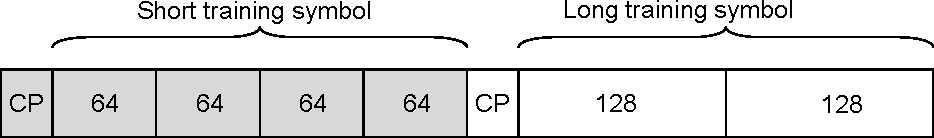
\includegraphics [width=0.7\columnwidth] {figures/Preamble.pdf} }
	\caption{Downlink preamble symbols for IEEE802.16.}
	\label{fig:pre}
\end{figure}

\begin{figure}
	\centerline{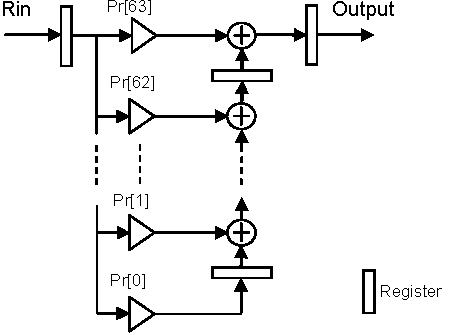
\includegraphics [width=0.5\columnwidth] {figures/structure_correlator.pdf} }
	\caption{Transpose Direct Form of Correlator.}
	\label{fig:str_corr}
\end{figure}


The 64 samples in the short symbol are used to perform cross-correlation with received samples for timing synchronisation. 
Therefore, the correlators are designed to compute cross-correlation with 64 constant coefficients. 
In this chapter, we explore two approaches to implementing such correlators. 
The first is based on Xilinx Virtex-6 FPGA DSP48E1 Slices, the standard approach to such an implementation.
The second is using multiplierless correlation implemented on both a Xilinx Virtex-6 and a low power Xilinx Spartan-6 device.
Both are designed to receive real and imaginary 16-bit samples in Q1.15 fixed point format. 
The output is the sum of 64 coefficient products, each being smaller than unity. 
So, the complex output words are in 21-bit fixed point Q6.15 format. 

If such a design was implemented blindly, with no consideration for the FPGA architecture, the synthesis tools would infer the use of embedded DSP blocks for multiplication, but would likely achieve poor timing due to an inability to optimise the use of the DSP block.
The DSP48E1 primitives on the Virtex-6 FPGAs have additional circuitry within them that enables the design of optimised datapaths, but this must be done manually, through writing code in a particular style.
Otherwise, the synthesis tools cannot always infer the most efficient structure.
In our design, we have taken into account the internal structure of the DSP block, and made the design as lean as possible.
The multiplierless design is specified entirely manually, and thus cannot be inferred by the tools.

%---------------------------------------------------------------------------------
\subsection{Design of DSP48E1 Based Correlator}

The DSP48E1 Slice inside the Virtex-6 shown in Fig. \ref{fig:DSP48E1} contains a multiplier followed by a configurable arithmetic unit to provide many independent functions, e.g., multiply, multiply accumulate, multiply add, three-input add, and more \cite{Xilinx2011}.
It also allows the datapath to be configured for various imput combinations and register stages; a three-stage pipeline offers maximum performance.
Since the DSP Slice is designed to mirror the structure of an FIR filter tap, it is ideally suited to implement correlation, and would hence be the method of choice for this application. 
Our first design uses non-pipelined DSP48E1 Slices in transpose direct form, as shown in Fig. \ref{fig:str_corr}, with 64 coefficients corresponding to the 64 samples in the preamble. 
The coefficients are pre-computed according to the IEEE802.16d standard. 
The second design spreads the complex multiply-adds in a five-stage pipeline, shown in Fig. \ref{fig:Cmp_MultAdder}, consisting of DSP48E1 Slices configured for three stage internal pipelining.  
$Ri\_Re$, $Ri\_Im$ are the real and imaginary parts of received sample, respectively. 
$Pr\_Re$, $Pr\_Im$ similarly represent known preamble. 
The pipeline registers for the $Pr\_Re$, $Pr\_Im$ are eliminated because they are considered to be of constant value. 
$Re$, $Im$ are the real and imaginary parts of the previous multiply-add. 
Fig. \ref{fig:DSP48pp_correlator} presents the pipeline structure of the correlator. 
The additional pipeline registers are required for handling the received sample.
Adding pipeline registers should increase performance significantly.
\begin{figure}
	\centerline{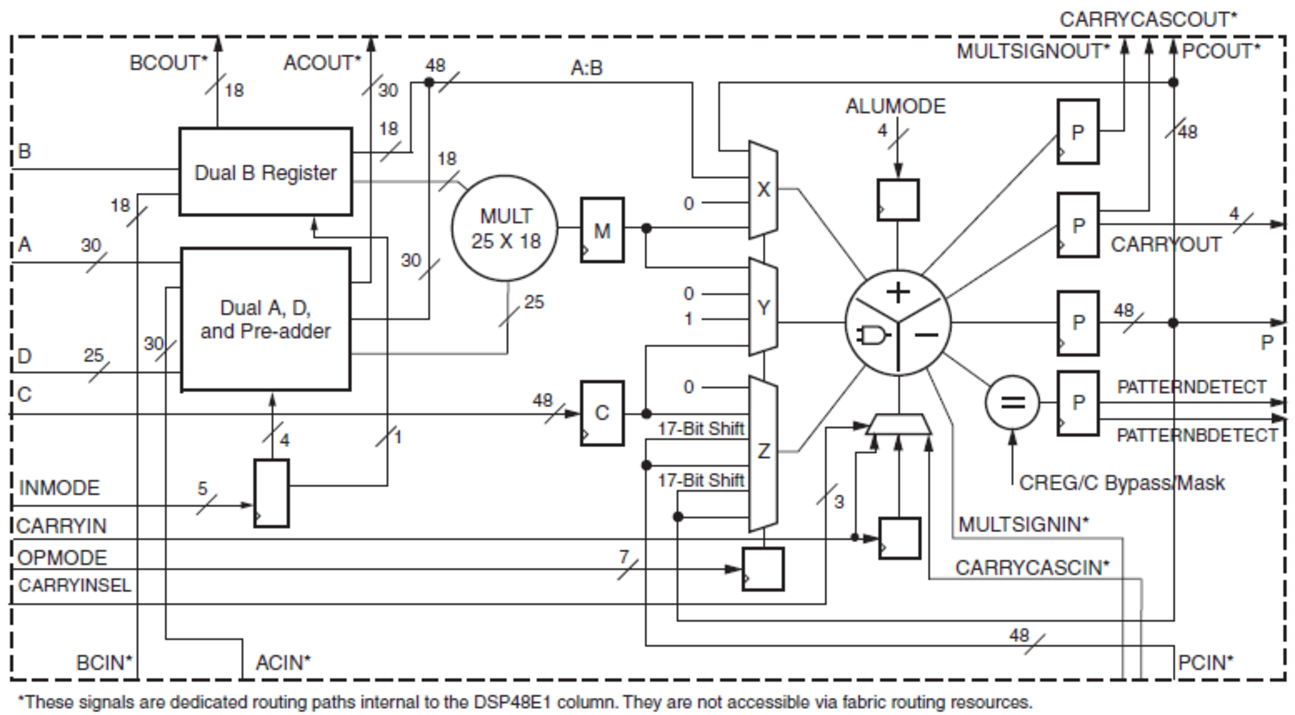
\includegraphics [width=0.9\columnwidth] {figures/DSP48E1.pdf} }
	\caption{Structure of DSP48E1 slice inside the Virtex-6 \cite{Xilinx2011}}
	\label{fig:DSP48E1}
\end{figure}

\begin{figure}
	\centerline{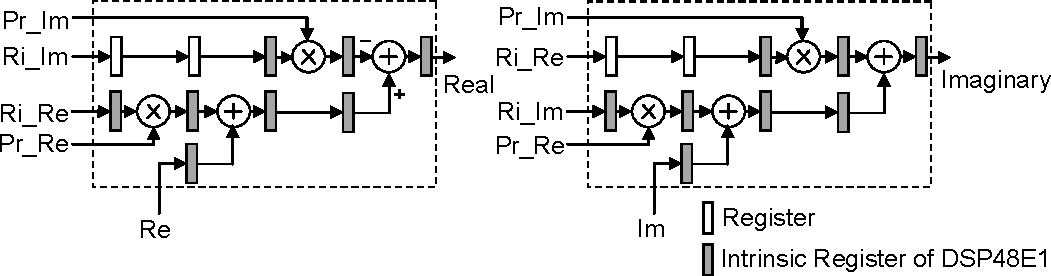
\includegraphics [width=0.9\columnwidth] {figures/Cmp_MultAdder.pdf} }
	\caption{Pipeline structure of the complex number multiply-add.}
	\label{fig:Cmp_MultAdder}
\end{figure}

\begin{figure}
	\centerline{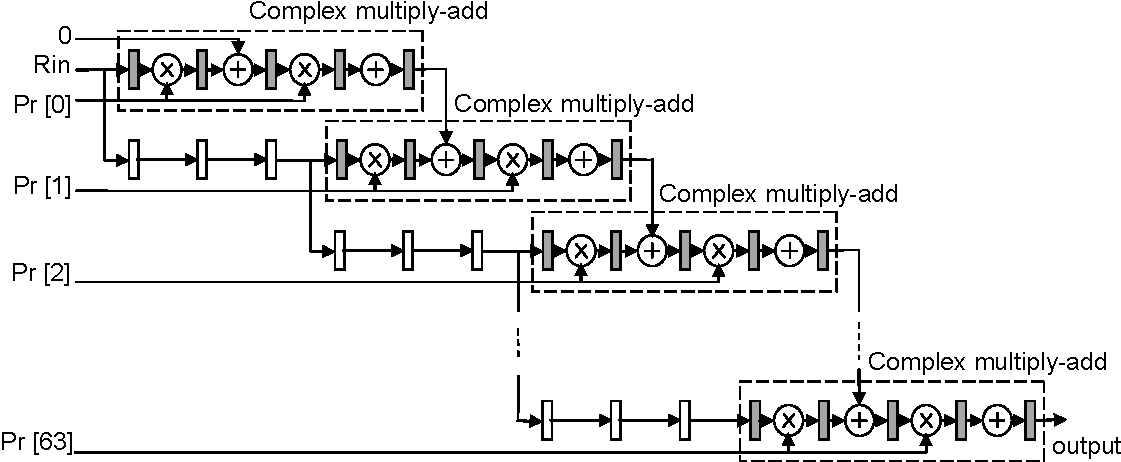
\includegraphics [width=0.9\columnwidth] {figures/DSP48pp_correlator.pdf} }
	\caption{Pipeline structure of correlator using DSP48E1 Slices.}
	\label{fig:DSP48pp_correlator}
\end{figure}

\begin{figure}
	\centerline{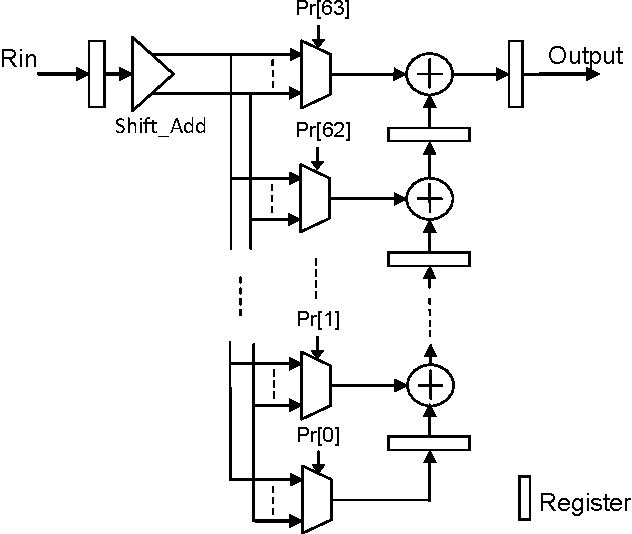
\includegraphics [width=0.7\columnwidth] {figures/ML_correlator.pdf} }
	\caption{Structure of multiplierless correlators.}
	\label{fig:ML_correlator}
\end{figure}

%---------------------------------------------------------------------------------
\subsection{Design of Multiplierless Correlator}

The principle of multiplierless correlators is to represent the coefficients and round them in the form of summed powers of two. 
Hence, a shift and add are performed instead of multiplying by coefficients. 
It is expected that multiplierless correlation is more efficient, but with embedded hard multipliers in modern FPGAs, it is unclear whether they should still be considered favourable. 
Furthermore, synchronisation accuracy must be considered.
To explore this, four alternative multiplierless correlators are implemented using four coefficient sets with an increasing degree of rounding, to compare the cost and performance and evaluate against multiplier-based correlators. 
The coefficient sets are found by quantising the 64 normalised preamble samples with quantisations of 1, 0.5, 0.25, and 0.125. 

The proposed structure for multiplierless correlators is shown in Fig. \ref{fig:ML_correlator}. 
This structure is based on the transpose-direct-form in Fig. \ref{fig:str_corr}. 
Instead of using multipliers to multiply input samples by coefficients, the $Shift\_Add$ block and multiplexers are used to perform the equivalent operation without an actual multiplication. 
But the  $Shift\_Add$ block, multilexers and value of $Pr[n]$ are different depending upon the quantised coefficient set being used.  
The $Shift\_Add$ block performs shift and add on received samples according to the degree of quantisation that is applied.  
To optimise resources in the case of small numbers of bit quantisation, one common $Shift\_Add$ block is used for all 64 coefficients instead of 64 separate $Shift\_Add$ blocks. 
This common $Shift\_Add$ block calculates all possible values for 64 coefficients.  
The multiplexers are used to select the corresponding values from $Shift\_Add$ to accumulate in order to generate the correlator output.
These are based on expressed coefficients $Pr[n]$ that are pre-computed based on quantizing the 64 preamble samples.
Since the $Pr[n]$ values are constants, after synthesising the design, the multiplexer is optimised as hard-wired logic, and the preamble cannot be changed.
To support different OFDM preambles, the $Pr[n]$ could be stored in a register, and a real multiplexer used instead of hard-wired logic.  
This results in increased resource utilisation but provides a more flexible solution. 

\subsection{Implementation Results}

The designs presented were synthesised and fully implemented using Xilinx ISE 13.2, targetting Xilinx Virtex-6 (V6) and Spartan-6 (S6) devices.  
The results of implementation are reported in terms of the number of occupied slices, DSP48E1s Slices and maximum frequency as summarised in Table \ref{tab:Imp_Rpt}. 

% Virtex-6 75T & Spartan-6 75T
\begin{table}[h]
	\centering
	\caption{Implementation Report}
	\label{tab:Imp_Rpt}
	\begin{tabular}{c|r|r|r|c|c}
        \hline \hline
    			Design  & \multicolumn{2}{|c|}{Occupied Slices} & DSP48E1s & \multicolumn{2}{|c}{Freq. (MHz)} \\
	\cline{2-6}			         & \makebox[1.2cm][c]{V6} & \makebox[1.2cm][c]{S6}& 	\makebox[1.2cm][c]{V6}	&  V6 & S6    \\
    	\hline
			DSPc 	& 742 		(6\%)  & -  			 & 256 (88\%) & 119 & -\\
			DSP\_pp &  1,110 	(9\%) & -  			 &  256 (88\%)& 398 & -\\
 			ML1 	&  661		(5\%) &	762 (6\%)	 &  0 (0\%)	& 309 & 174\\
			ML2 	&  983 	(8\%) &	1,071 (9\%) &  0 (0\%)	& 268 & 158\\
			ML3 	&  1,191 	(10\%) &	1,257 (10\%) &  0 (0\%)	& 234 & 136\\
			ML4 	&  1,496 	(12\%) &	1,517 (13\%) &  0 (0\%)	& 208 & 124\\   
    
    	\hline \hline  
    \end{tabular}	
\end{table}

$DSPc$, $DSP\_pp$ are correlator designs using DSP Slices, in non-pipelined and pipelined structures, respectively. 
$ML1$, $ML2$, $ML3$, $ML4$ are multiplierless correlators with coefficient quantisations of 1, 0.5, 0.25, 0.125, respectively.

Table \ref{tab:Imp_Rpt} reveals that the $DSP\_pp$ uses more logic slices due to its pipeline structure. 
The slices in DSP48E1 based designs are used for registers and route-thrus while the slices in the multiplierless designs are mostly used as logic. 
The number of slices used in the multiplierless designs increases as the coefficient quantisation becomes finer. 
The DSP48E1-based designs use 256 DSP Slices, 4 for each complex multiply plus 6-9\% of logic resources.
The multiplierless designs use only logic to compute the cross correlation with 64 complex coefficients. 
The total logic area is a small fraction of the whole device: around 5-12\% of total resources in the Virtex-6, and around 6-13\% of total resources in the equivalent Spartan-6.
While Spartan-6 devices do include DSP Slices, their number is insufficient to implement the full 64 sample complex cross correlation.
This shows an ideal scenario where multiplierless correlation makes sense, and hence serves as a motivation for this study.

The maximum frequencies, reported after place and route, decrease for multiplierless designs according to the degree of coefficient quantisation. 
Meanwhile the non-pipelined DSP48E1 design is slower than the multiplierless designs. 
However, the pipelined DSP48E1 design can achieve higher frequency.

A post-place-and-route simulation in ModelSim was used to estimate the power consumption of the system using the Xilinx XPower tool. 
Table \ref{tab:PWR} shows the power dissipation of the designs running at 50{\thinspace}MHz. 
The DSP48E1-based correlators consume more power than the multiplierless correlators, but this is due primarily to increased dynamic power when using the DSP48E1s on the Virtex-6. 
The dynamic power of the non-pipelined DSP48E1-based correlator $DSP\_Cor$ is greatest at 846{\thinspace}mW, but pipelining reduces this by a factor of more than 2.5 times, due to reduced switching activity between the multiplier and adder.  
The dynamic power of the multiplierless designs increases from 133{\thinspace}mW to 203{\thinspace}mW on Virtex-6 and from 149{\thinspace}mW to 294{\thinspace}mW on Spartan-6 as finer coefficient quantisation is used. 
It is important to note that the quiescent power of the Spartan-6 is much lower by design. 
Hence, we can see that using this multiplierless technique allows us to implement synchronisation on a Spartan-6 device, where a multiplier-based design is not possible, saving significant power and sacrificing little in terms of accuracy.

 % Virtex-6 75T  &  Spartan-6 75T
\begin{table}[h]
	\centering
	\caption{Power Consumption at 50MHz.}
	\label{tab:PWR}
	\begin{tabular}{c|c|c|c|c|c|c}
        \hline \hline
    			Correlators  & \multicolumn{2}{|c|}{Quiescent(mW)} &  \multicolumn{2}{|c|}{Dynamic(mW) }& \multicolumn{2}{|c}{Total(mW)} \\
	\cline{2-7}			& V-6 & S-6 & V-6 & S-6 & V-6 & S-6\\
	\hline
			DSP\_Cor		&  1312 &  -  	 & 846 & -	& 2158 &-\\
			DSP\_pp\_Cor 	& 1300  &  -   & 328 & - 	& 1628 & -\\
 			ML1\_Cor 		& 1296  & 67 & 133 & 149	& 1429 & 216\\
			ML2\_Cor 		& 1296  & 68 & 160 & 197	& 1456 & 265\\	
			ML3\_Cor 		& 1297  & 70 & 182 & 239	& 1479 & 309\\
			ML4\_Cor 		& 1297  & 71 & 203 & 294    & 1500 & 365\\   
    
    	\hline \hline  
    \end{tabular}
\end{table}


\begin{figure}
	\centerline{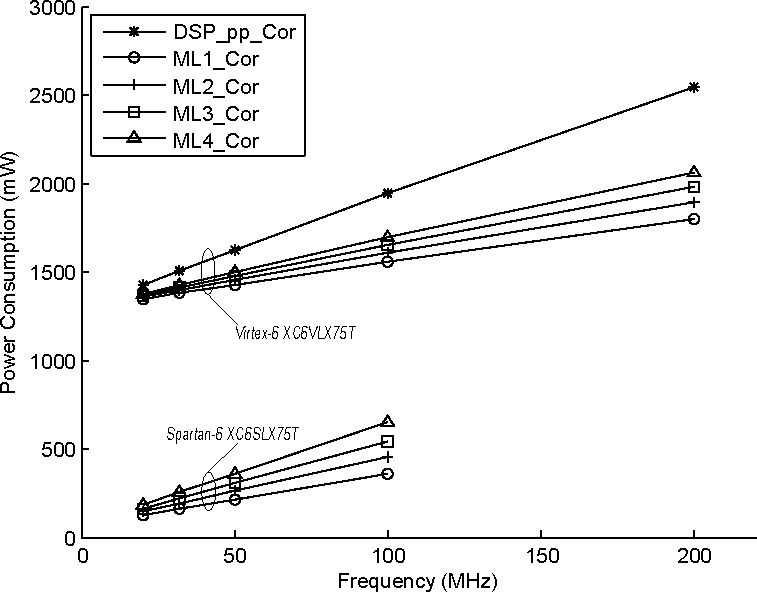
\includegraphics [width=0.9\columnwidth] {figures/Plot_PWR.pdf} }
	\caption{Power consumption of designs.}
	\label{fig:Plot_PWR}
\end{figure}

We also investigated how total power consumption varies with frequency, as shown in Fig. \ref{fig:Plot_PWR}.
As frequency increases, the finer quantisations and DSP48E1-based designs begin to consume proportionally more power.
Overall, multiplierless designs on the Spartan-6 consume 75\% to 85\% less power than the same designs on the Virtex-6, and a 0.25 quantisation design on the Spartan-6 consumes 81\% to 85\% less power then the DSP48E1-based design on a Virtex-6.

The \emph{DPS\_Cor} implementation represents how a ``blind'' design would be mapped. Our architecture-aware designs show significantly better performance, reduced area, and reduced power consumption.

%---------------------------------------------------------------------------------
\section{Simulation and discussion}
%---------------------------------------------------------------------------------
In order to validate our designs at the application level, we simulate them using ModelSim with an IEEE802.16 OFDM frame created using MATLAB, including the preamble symbols, data symbols and effects of an AWGN channel. 
Cross-correlation results using the correlator designs are compared to corresponding results in MATLAB to verify the correctness of implementation. 
To evaluate the accuracy of timing synchronisation acheivable by these designs, the correlation outputs are plotted in Fig. \ref{fig:Plot_XCR} for random data frames at 10{\thinspace}dB SNR. 
The output of each correlator is slightly different because of rounding, but the timing synchronisation depends upon the location of the peaks being at the  position of the preamble.
All the correlator designs achieve this most of the time, as shown at indices 34 and 98 for the CP samples and the first preamble samples respectively, for a single frame. 
 
\begin{figure}
	\centerline{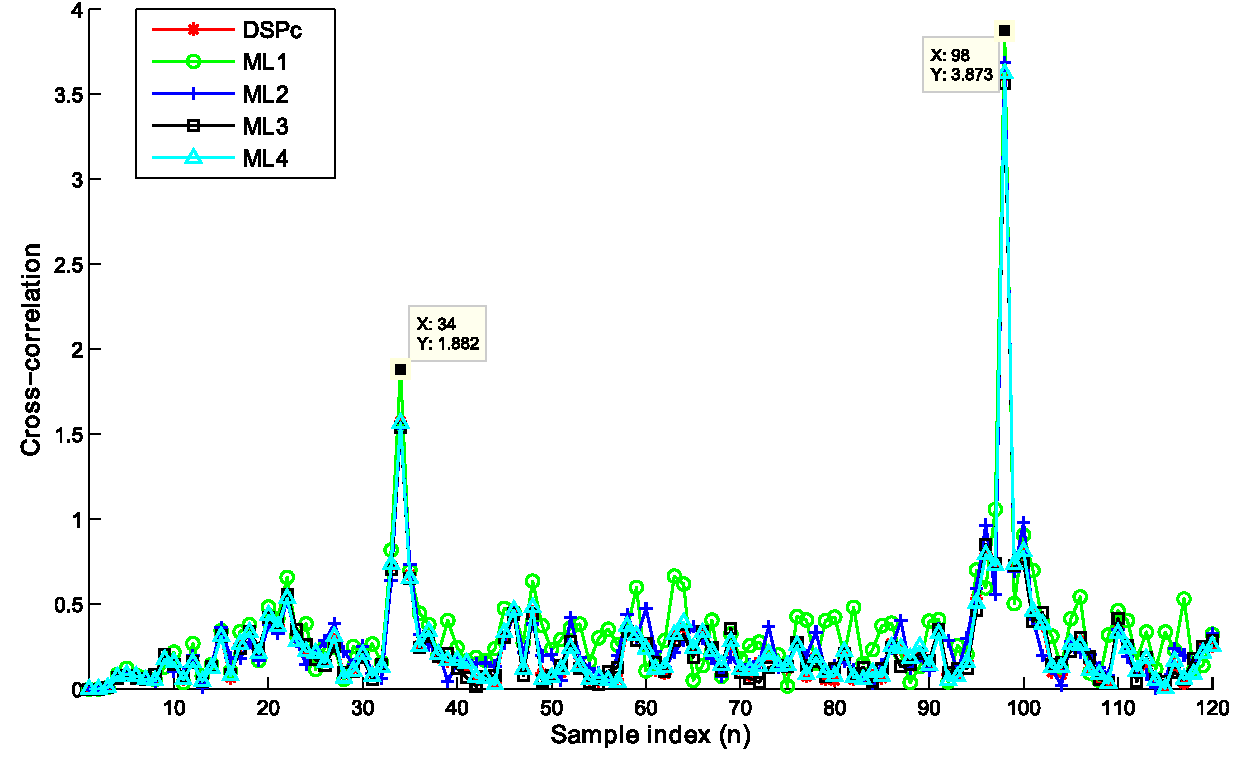
\includegraphics [width=0.9\columnwidth] {figures/Plot_XCR.pdf} }
	\caption{Correlator output with SNR = 10dB.}
	\label{fig:Plot_XCR}
\end{figure}

In order to evaluate the synchronisation accuracy of these approaches, we simulate 10,000 correlation operations in an AWGN channel with a detection strategy as follows. 
First, find the first peak, $P1$, over 64 samples. 
Next, find the second peak, $P2$, in the next 64 samples from the first peak and compute average value, $avg$, of the samples between two peaks. 
If  $( P1 - avg ) \le  0.75 * ( P2 - avg )$, the start of frame is detected and the correctness of the position can be checked. 
It should be noted that in all cases, the peaks were known to be located within the two search regions and that the detection strategies described above are compatible with those of other authors such as \cite{Kishore2006} and \cite{Yip2003}. 
Fig. \ref{fig:Plot_NFail} plots the results in terms of failure rate against AWGN SNR and show that the designs are able to accurately detect the start of frame even in low SNR conditions. 
The failure rate of $ML1\_Cor$ is the highest, as expected, due to the coarse quantisation.
For SNRs above 4{\thinspace}dB, the failure rates of $ML2\_Cor$, $ML3\_Cor$,  $ML4\_Cor$ and $DSP\_Cor$ differ less than 0.05\% from each other.
This suggests that sacrificing accuracy by using multiplierless cross-correlation is feasible and has negligible impact on synchronisation accuracy.
Combined with the results in the previous section, we can be confident that low-power FPGAs, such as the Spartan-6, with insufficient resources for multiplier-based synchronisation correlation, are still feasible for implementing robust OFDM receivers.

\begin{figure}
	\centerline{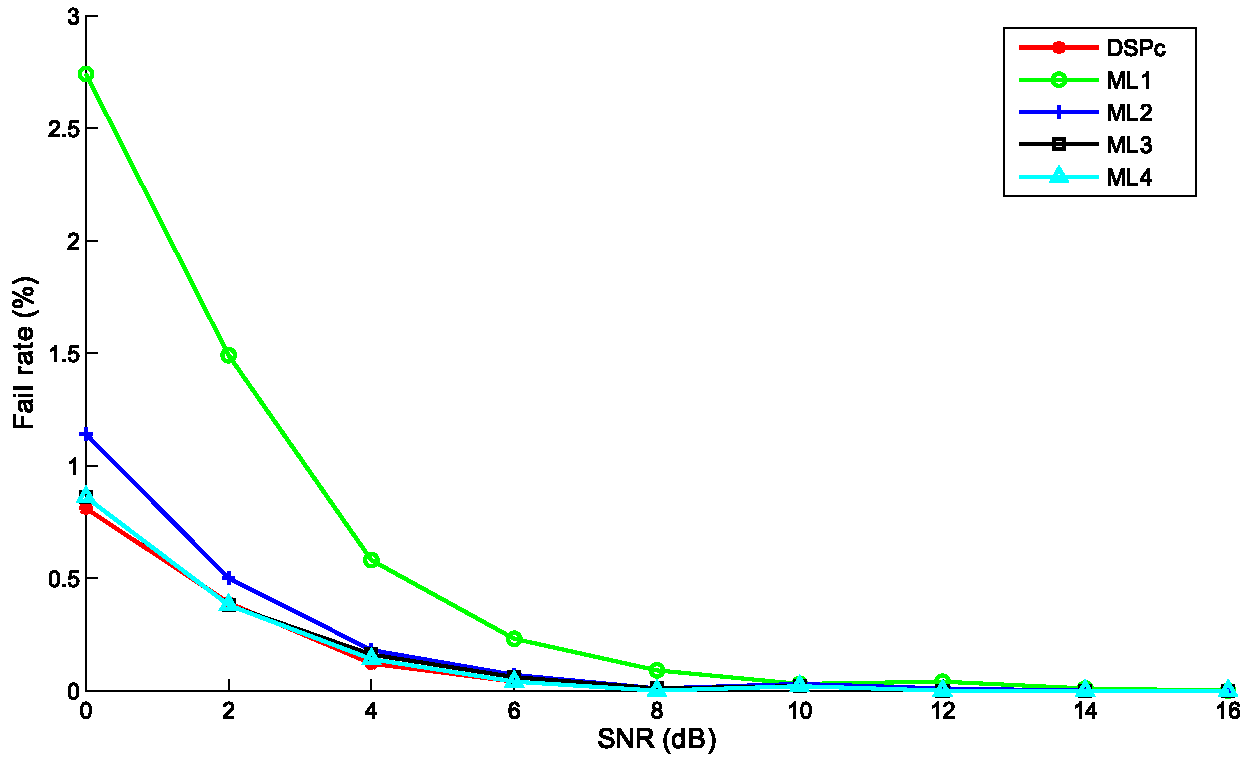
\includegraphics [width=0.85\columnwidth] {figures/Plot_NFail.pdf} }
	\caption{Detection failure rate.}
	\label{fig:Plot_NFail}
\end{figure}

%---------------------------------------------------------------------------------
\section{Summary}
%---------------------------------------------------------------------------------
The DSP48E1 Slices on modern Virtex-6 FPGA devices seem to offer the ideal resource for implementing correlation-based frame synchronisers.
However, as we have discovered, in the context of synchronisation for IEEE802.16 OFDM systems, simplified multiplierless designs offer comparable synchornisation performance. 
While the DSP48E1-based correlators can obtain higher clock speeds, this is only possible through a detailed pipelined design.
Furthermore, their power consumption and resource usage is considerably greater.
Since low-power, low-cost devices such as the Xilinx Spartan-6 do not include sufficient DSP Slices, this suggests adopting multiplierless designs for low-power implementations.
We have shown that while very low quantisation resolution does impact synchronisation performance, with a step size of just 0.5, synchronisation accuracy is on par with multiplier-based correlation. 
Multiplierless correlation on a Spartan-6 can save over 85\% power compared to  a DSP Slice design on a Virtex-6 FPGA.

This work has been submitted as a journal paper to  IEEE transactions on Very Large Scale Integration (VLSI) systems.
\chapter{Multiplierless Correlator Design for low-power systems}
\label{chap:multiplierlesscorrelator}
	\section{Introduction}
	\section{Implementation of correlators}
		\subsection{Design of DSP48E1 Based Correlator}
		\subsection{Design of Multiplierless Correlator}
		\subsection{Implementation Results}
	\section{Simulation and discussion}
	\section{Summary}
%\include{ch4-Synchronisation}
\chapter{Proposed Method for OFDM Synchronisation}
\label{chap:Synchronisation}
	\section{Introduction}
	\section{Proposed Technique for FFO and STO Estimation}
	\section{Enhanced Synchronization Through Novel IFO Estimation Architecture}
	\section{Summary}
%\include{ch5-SpectralLeakage}
\chapter{Proposed Method for Shaping OFDM Spectral Leakage}
\label{chap:SpectralLeakage}
	\section{Introduction}
	\section{Proposed Technique for Adaptive Shaping Spectral Leakage}
	\section{Simulation Results and Discussion}
	\section{Summary}
%\include{ch6-MSCR}
\chapter{A Novel Architecture for Multiple Standard Cognitive Radios}
\label{chap:MSCR}
	\section{Introduction}
	\section{Proposed OFDM-based baseband modulation for MSCR}
	\section{Performance Analysis and Discussion}
\section{Summary}
%\include{ch7-Conclusion}
\chapter{Conclusion and Future Work}
\label{chap:conclusion}




% -------------------------------------------------------------------------------- %
% --------------------------- Part III. The Back Matters ------------------------- %
% -------------------------------------------------------------------------------- %
\appendix
%%---------------------------------------------------------------------------------
\chapter{Appendix}
\label{chap:Appendix}
%---------------------------------------------------------------------------------
\section{Kronecker Product}\label{appen:Kronecker}
The Kronecker product is also called matrix direct product and is
usually represented as $\otimes$. For example, the Kronecker product
a $2\times2$ matrix $A$ and a $3\times2$ matrix $B$ is define as
\begin{eqnarray}\label{Kronecker}
    A\otimes B &=& \left(%
\begin{array}{cc}
  a_{11}B & a_{12}B \\
  a_{21}B & a_{22}B \\
\end{array}%
\right)\nonumber\\
&=&\left(%
\begin{array}{cccc}
  a_{11}b_{11} & a_{11}b_{12} & a_{12}b_{11} & a_{12}b_{12} \\
  a_{11}b_{21} & a_{11}b_{22} & a_{12}b_{21} & a_{12}b_{22} \\
  a_{11}b_{31} & a_{11}b_{32} & a_{12}b_{31} & a_{12}b_{32} \\
  a_{21}b_{11} & a_{21}b_{12} & a_{22}b_{11} & a_{22}b_{12} \\
  a_{21}b_{21} & a_{21}b_{22} & a_{22}b_{21} & a_{22}b_{22} \\
  a_{21}b_{31} & a_{21}b_{31} & a_{22}b_{31} & a_{22}b_{32} \\
\end{array}%
\right)
\end{eqnarray}
The result is a $6\times4$ matrix, where any elements from the $A$
is multiplied with any elements from $B$. For general case, the
Kronecker product of a $M\times N$ matrix $A$ and a $P\times Q$
matrix $B$, the resulting matrix is $MP\times NQ$, and the elements
of the resulting matrix is defined as
\begin{equation}\label{Kronecker2}
    c_{\alpha,\beta}=a_{ij}b_{kl}
\end{equation}
where
\begin{eqnarray}
% \nonumber to remove numbering (before each equation)
  \alpha &=& P(i-1)+k \\
  \beta &=& Q(j-1)+l
\end{eqnarray}
      % Appendix and Publications
%\chapter* {Publication}
\addcontentsline{toc}{chapter}{\numberline{}\hspace{-0.24in}{\bf
Publication}}




% Include the references
\newpage
\addcontentsline{toc}{chapter}{References}
\bibliographystyle{ieeetr}      % Use the IEEE bibiography style
\bibliography{ConfirRpt_macro,ConfirRpt}  % Include the BibTex files





\end{document}      % End of the text



% ------------------
% End of the File
% ------------------
